% SIAM Article Template
% `nohypdvips` lets the document compile with XeTeX/tectonic (the class otherwise loads the
% dvips-only hypdvips package); it is harmless under pdfLaTeX, where that branch is not taken.
\documentclass[review,onefignum,onetabnum,nohypdvips]{siamonline250211}
% Information that is shared between the article and the supplement
% (title and author information, macros, packages, etc.) goes into
% ex_shared.tex. If there is no supplement, this file can be included
% directly.

% SIAM Shared Information Template
% This is information that is shared between the main document and any
% supplement. If no supplement is required, then this information can
% be included directly in the main document.


% Packages and macros go here
\usepackage{lipsum}
\usepackage{amsfonts}
\usepackage{graphicx}
\usepackage{caption}
\usepackage{subfig}
\usepackage{epstopdf}
\usepackage{algorithmic}
\usepackage{booktabs}
\ifpdf
  \DeclareGraphicsExtensions{.eps,.pdf,.png,.jpg}
\else
  \DeclareGraphicsExtensions{.eps}
\fi

% Prevent itemized lists from running into the left margin inside theorems and proofs
\usepackage{enumitem}
\setlist[enumerate]{leftmargin=.5in}
\setlist[itemize]{leftmargin=.5in}

% Add a serial/Oxford comma by default.
\newcommand{\creflastconjunction}{, and~}

% Used for creating new theorem and remark environments
\newsiamremark{remark}{Remark}
\newsiamremark{hypothesis}{Hypothesis}
\newsiamremark{assumption}{Assumption}
\crefname{hypothesis}{Hypothesis}{Hypotheses}
\newsiamthm{claim}{Claim}
\newsiamremark{fact}{Fact}
\crefname{fact}{Fact}{Facts}

% Sets running headers as well as PDF title and authors
\headers{An Iterative Network for Parameter Estimation in Nonlinear Dynamical Systems from Sparse and Partial Observations}{Seong-heon Lee, Dongjin Lee, Jiaxi Gu, Joon Ha, and Jae-Hun Jung}

% Title. If the supplement option is on, then "Supplementary Material"
% is automatically inserted before the title.
\title{An Iterative Network for Parameter Estimation in Nonlinear Dynamical Systems from Sparse and Partial Observations\thanks{Submitted to the editors DATE.
\funding{This work was funded by the Fog Research Institute under contract no.~FRI-454.}}}

% Authors: full names plus addresses.
\author{
  Seong-Heon Lee\thanks{Graduate School of Artificial Intelligence, POSTECH, Pohang, Republic of Korea 
    (\email{shlee0125@postech.ac.kr}, \email{dongjinlee@postech.ac.kr}).}
  \and
  Dongjin Lee\footnotemark[2]
  \and
  Jiaxi Gu\thanks{Department of Mathematics, POSTECH, Pohang, Republic of Korea 
    (\email{jiaxigu@buffalo.edu}, \email{jung153@postech.ac.kr}).}
  \and
  Joon Ha\thanks{Department of Mathematics, Howard University, Washington, DC 20059, U.S.A. 
    (\email{joon.ha@Howard.edu}).}
  \and
  Jae-Hun Jung\footnotemark[3]
}

\usepackage{amsopn}
\DeclareMathOperator{\diag}{diag}

% ===== Hyperparameter highlighting (draft mode) =====
\newif\ifhpcolor
\hpcolortrue % draft: true, final submission: false

\ifhpcolor
  \usepackage{xcolor}
  \newcommand{\HP}[1]{\textcolor{blue}{#1}}
\else
  \newcommand{\HP}[1]{#1}
\fi

% ---------- Hyperparameter value macros ----------
\newcommand{\HPSys}{\HP{ogtt\_simul}}
\newcommand{\HPSeed}{\HP{42}}
\newcommand{\HPNumSamples}{\HP{10000}}
\newcommand{\HPAugFactor}{\HP{30}}
\newcommand{\HPTestSplit}{\HP{0.2}}
\newcommand{\HPBatchSize}{\HP{512}}

\newcommand{\HPEpochs}{\HP{10000}}
\newcommand{\HPLR}{\HP{1e-4}}
\newcommand{\HPWeightDecay}{\HP{1e-4}}
\newcommand{\HPEarlyStop}{\HP{True}}
\newcommand{\HPEarlyPat}{\HP{200}}
\newcommand{\HPEarlyDelta}{\HP{1e-6}}

\newcommand{\HPUseDeriv}{\HP{True}}
\newcommand{\HPDerivMethod}{\HP{spline}}
\newcommand{\HPIter}{\HP{10}}

\newcommand{\HPLossCfg}{\HP{supervised + recurrent (equal weights)}}

\newcommand{\HPHiddenDims}{\HP{[64,64,64]}}
\newcommand{\HPAct}{\HP{SiLU}}
\newcommand{\HPSN}{\HP{True}}

\newcommand{\HPSDEBias}{\HP{1.0}}
\newcommand{\HPSDEDiff}{\HP{1.27}}

%%% Local Variables: 
%%% mode:latex
%%% TeX-master: "ex_article"
%%% End: 


% Optional PDF information
\ifpdf
\hypersetup{
  pdftitle={An Iterative Network for Parameter Estimation in Nonlinear Dynamical Systems from Sparse and Partial Observations},
  pdfauthor={Seong-heon Lee, Dongjin Lee, Jiaxi Gu, and Jae-Hun Jung}
}
\fi

% The next statement enables references to information in the
% supplement. See the xr-hyperref package for details.

\externaldocument[][nocite]{ex_supplement}

% FundRef data to be entered by SIAM
%<funding-group specific-use="FundRef">
%<award-group>
%<funding-source>
%<named-content content-type="funder-name"> 
%</named-content> 
%<named-content content-type="funder-identifier"> 
%</named-content>
%</funding-source>
%<award-id> </award-id>
%</award-group>
%</funding-group>

\begin{document}

\maketitle

% REQUIRED
\begin{abstract}
Estimating parameters of nonlinear dynamical systems from sparse and partial observations is a
severely ill-posed inverse problem. A natural and appealing strategy is to \emph{decouple} it: learn
one network that reconstructs the unobserved (hidden) state from the observations and a current
parameter guess, and another that updates the parameter from the observations and the reconstructed
state, then iterate the composition to a fixed point. We study this decoupled fixed-point estimator
and give a complete characterization of what it can and cannot do. On the positive side, enforcing
Lipschitz bounds (e.g., by spectral normalization) makes the update a contraction, so the iteration
converges to a unique fixed point from any initialization at a geometric rate. On the limiting side,
we show that convergence does not deliver correctness, and that the limitation is structural rather
than a training artifact. Because the fixed point is a deterministic function of the observation, it
cannot beat the conditional-mean estimator---reconstructing the hidden state confers no information
advantage at inference, since the reconstructed state is itself a function of the observation---and a
plain direct regressor typically reaches this ceiling more closely. Under non-identifiability the
conditional mean is moreover displaced strictly off the manifold of parameters consistent with the
observation, so the squared-loss estimate is not even physically admissible. We predict the
identifiability of three benchmark systems (SIR, Lotka--Volterra, OGTT) a priori via a Hermann--Krener
observability analysis and confirm each prediction empirically. The results delineate a fundamental
ceiling for deterministic decoupled point estimation and motivate lifting inference from point
estimates to distributions.
\end{abstract}

% REQUIRED
\begin{keywords}
dynamical systems,
partial observation,
inverse problems,
parameter estimation,
non-identifiability,
machine learning,
neural networks
\end{keywords}

% REQUIRED
\begin{MSCcodes}

\end{MSCcodes}

\section{Introduction}

% Section 1: Introduction
%% Paragraph 1 : Issue
Estimating the governing parameters of nonlinear dynamical systems from time-series observations is a fundamental inverse problem with broad applications in epidemiology, ecology, and physiology. % TODO: citation (fundamental inverse problems) 
In many practical settings, however, observations are severely constrained: they are often \emph{partial} (only a subset of the state variables is measurable) and \emph{sparse} (a relatively small number of time points are observed). 
These physical constraints render the inverse mapping from observations to parameters highly ill-posed and, in certain regimes, structurally non-identifiable. 
When key states remain hidden, resolving these unobserved latent trajectories simultaneously with the system parameters formulates a joint optimization problem.
This coupling inherently creates a highly non-convex loss landscape, drastically amplifying the computational and theoretical difficulty.

% Paragraph 2 : Limitations of existing methods
Traditional approaches combine mechanistic numerical integration with optimization techniques, such as nonlinear least squares (NLLS) or sampling based method (MCMC). % TODO: citation (NLLS/MCMC textbooks)
While mathematically principled, these per-instance optimizations incur significant computational costs and are highly sensitive to initial conditions; 
they frequently fall into local minima or diverge when applied to sparse measurements of complex oscillatory or non-autonomous systems.

% Paragraph 3 : Propose our solution
To address these limitations, we propose a novel parameter estimation framework structured as a contractive fixed-point iteration. 
We first decouple the joint inverse problem into two conditional tasks: a hidden-state estimator infers the latent trajectory given partial observations and a parameter guess, while a parameter estimator updates the parameter vector given the observations and the inferred hidden state. 
Inference is then performed by alternating updates between these two trained neural networks. However, simply coupling two neural networks offers no theoretical guarantee of stability; the alternating sequence could easily oscillate or diverge. 
To overcome this, we enforce Lipschitz bounds on both networks via spectral normalization. 
This rigorous structural constraint guarantees that their composition forms a contraction mapping, ensuring that the inference iteration converges exponentially to a unique fixed point from any initialization.

% Paragraph 4 : Results
We demonstrate the effectiveness of this framework through extensive numerical evaluations on epidemiological (SIR), ecological (Lotka-Volterra), and physiological (OGTT) models. 
Our results show that the proposed fixed-point architecture robustly recovers parameters from sparse and partial data in regimes where traditional joint optimization fails. 
To provide a deeper understanding of these empirical outcomes, we utilize the Hermann-Krener nonlinear observability framework~\cite{hermann2003nonlinear} as an analytical tool. 
This theoretical grounding allows us to explicitly characterize identifiable regimes and provides a principled explanation for phenomena such as regression-to-mean (model collapse) encountered in structurally unidentifiable scenarios.

%\textbf{Contributions.} The main contributions of this paper are threefold:
%\begin{itemize}
%    \item We introduce a decoupled fixed-point iteration architecture that enables stable parameter inference from sparse and partial observations.
%    \item We provide a rigorous mathematical guarantee that the proposed iterative update acts as a contraction mapping, ensuring exponential convergence to a unique fixed point.
%    \item We empirically validate the framework on multiple nonlinear systems and provide a theoretical analysis of structural identifiability to clarify the boundaries of reliable parameter recovery.
%\end{itemize}
Parameter estimation for nonlinear dynamical systems from time-series observations is an inverse problem with broad scientific applications~\cite{tarantola2005inverse}. 
While parameter estimation is inherently ill-posed, practical constraints on data collection severely exacerbate this difficulty.
In practical settings, observations are frequently restricted:
the system state is only \emph{partially} observable, capturing a limited subset of the variables, and the temporal sampling intervals can become highly \emph{sparse}.
These limitations deprive the inverse mapping of critical information, frequently driving the system into non-identifiable regimes where distinct parameter values induce essentially indistinguishable observed trajectories.

A common approach is to treat inference as either (i) per-instance numerical optimization over parameters (and possibly latent states) or (ii) direct regression from observations to parameters using a machine learning model. 
While optimization-based methods are mathematically principled, they can be computationally expensive and sensitive to initialization in sparse regimes, and they may converge to different solutions when the inverse problem admits multiple nearly equivalent explanations. 
Regression-based approaches amortize inference cost by learning a direct map from observations to parameters. They are simple and, as our experiments confirm, a strong baseline; what they do not do is exploit the dynamical structure of the forward model or form any explicit estimate of the unobserved state. This gap motivates methods that reconstruct the latent trajectory as part of inference, on the intuition that using the hidden state should help --- an intuition whose limits this paper makes precise.

In this work, we adopt a fixed-point inference formulation that makes the inference dynamics explicit.
We represent sparse observations $\mathbf{x}_{\mathrm{obs}}$  and define a learned update operator $ \mathcal{T}(\theta;\mathbf{x}_{\mathrm{obs}})=P_{\psi}\left(\mathbf{x}_{\mathrm{obs}},H_{\phi}(\mathbf{x}_{\mathrm{obs}},\theta)\right)$, where $H_{\phi}$ is a hidden-state estimator and $P_{\psi}$ is a parameter estimator. 
Inference is performed by the fixed-point iteration $\theta^{k+1}=\mathcal{T}(\theta^{k};\mathbf{x}_{\mathrm{obs}})$, and the final prediction is the fixed point $\theta^*(\mathbf{x}_{\mathrm{obs}})$. 
The key design objective is contractivity of $\mathcal{T}(\cdot;\mathbf{x}_{\mathrm{obs}})$ for each fixed $\mathbf{x}_{\mathrm{obs}}$, which guarantees global convergence to a unique fixed point with a geometric rate.

Crucially, convergence does not imply correctness, and analyzing \emph{what} the fixed point is turns out to yield a characterization of a fundamental limitation rather than a guarantee of accuracy. Because the fixed point is a deterministic function of $\mathbf{x}_{\mathrm{obs}}$, it cannot be more accurate than the conditional mean $\mathbb{E}[\theta\mid\mathbf{x}_{\mathrm{obs}}]$; in particular, reconstructing the hidden state --- the feature that motivates the decoupling --- confers no information advantage at inference, since the reconstructed state is itself an image of $\mathbf{x}_{\mathrm{obs}}$. The deviation of the fixed point from this conditional-mean ceiling is controlled by a one-step residual $\varepsilon(\mathbf{x}_{\mathrm{obs}})=\lVert \mathcal{T}(\theta^{\mathrm{true}};\mathbf{x}_{\mathrm{obs}})-\theta^{\mathrm{true}}\rVert$, which we bound and decompose into a structural part and an operator-approximation part.

The consequence is sharpest under non-identifiability, where the conditional mean is not merely inaccurate: for a curved solution fiber it lies strictly \emph{off} the manifold of parameters consistent with the observation, so the squared-loss estimate is not even physically admissible. This regression-to-the-mean and joint-distribution collapse persists no matter how well the iteration converges; it reflects the information content of the observations and the choice of supervised loss, not a numerical artifact. Taken together, our results say that a decoupled deterministic point estimator, however well-motivated and however stably it converges, is bounded by the (off-fiber) conditional mean --- a limitation that motivates lifting inference from point estimates to distributions.

Our main contributions are:
\begin{itemize}
    \item We formulate parameter estimation from sparse partial observations as a fixed-point problem in parameter space, defined by an update operator $\theta^{(i+1)}=\mathcal{T}(\theta^{(i)};\mathbf{x}_{\mathrm{obs}})$ composed of a hidden-state estimator and a parameter estimator.
    \item We provide a sufficient condition for $\mathcal{T}(\cdot;\mathbf{x}_{\mathrm{obs}})$ to be contractive and hence globally convergent to a unique fixed point with a geometric rate, and we show how to enforce the required Lipschitz bounds in practice (e.g., via spectral normalization).
    \item  We separate convergence from correctness and characterize the fixed point: it is a function of $\mathbf{x}_{\mathrm{obs}}$ and therefore cannot beat the conditional-mean ceiling $\mathbb{E}[\theta\mid\mathbf{x}_{\mathrm{obs}}]$ (reconstructing the hidden state adds no information at inference); its deviation from that ceiling is bounded by a one-step residual $\varepsilon(\mathbf{x}_{\mathrm{obs}})$, which we decompose into a structural and an operator-approximation part.
    \item We show that under non-identifiability the conditional mean is itself displaced off the physical solution fiber (a Jensen/extreme-point argument), so squared-loss point estimation yields a physically inadmissible estimate; this regression-to-the-mean and joint-distribution collapse persists regardless of convergence.
    \item On epidemiological (SIR), ecological (Lotka--Volterra), and physiological (OGTT) systems, whose identifiability we predict a priori by a Hermann--Krener observability analysis, we confirm each prediction empirically --- including that a direct regressor reaches the conditional-mean ceiling more closely than the decoupled iteration, isolating the cost of the reconstruction detour.
\end{itemize}

% Section 2: Related Works
%\section{Related Works}
\label{sec:related_works}
%latent state/partial observation system ID, PINNs, neural ODE, filtering/EM류
%contractive nets / Lipschitz control
%identifiability/observability (Herman–Krener)


To be written....

% Sect0ion 3: Problem Formulation
\section{Problem Formulation}
\label{sec:problem}

In this section, we formally define the problem of parameter estimation for dynamical systems under \emph{partial and sparse observation} settings. 
Let $\mathbf{x}(t)\in\mathbb{R}^d$ denote the full state of the dynamical system and $\theta\in\Theta\subset\mathbb{R}^p$ the unknown parameter vector.
The underlying dynamics are governed by the ordinary differential equation (ODE)
\begin{equation}
\label{eq:ode}
    \dot{\mathbf{x}}(t)=f(\mathbf{x}(t),\theta),\qquad t\in[0,T],
\end{equation}
where $f:\mathbb{R}^d\times\Theta\to\mathbb{R}^d$ is a known, sufficiently smooth vector field.
The classical parameter estimation problem seeks to infer the unknown parameter $\theta$ given the continuous trajectory of the full state $\mathbf{x}(t)$~\cite{tarantola2005inverse}. 
In practical applications, however, obtaining such complete observations is rarely feasible.
The following subsections define the specific constraints of realistic observations and formulates the resulting inverse problem.

\subsection{Partial and Sparse Observation Setting}
\label{subsec:obsmodel}

We consider a \emph{partial observation} setting, in which only a subset of the state variables is observable.
We decompose the full state $\mathbf{x}(t)$ into an \emph{observed} state $x_{\mathrm{obs}}(t)\in\mathbb{R}^{d_{\mathrm{obs}}}$ and a
\emph{unobserved} state $x_{\mathrm{hid}}(t)\in\mathbb{R}^{d_{\mathrm{hid}}}$, such that $d_{\mathrm{obs}}+d_{\mathrm{hid}}=d$.
We refer to this unobserved state as the \emph{hidden state}. Reconstructing it explicitly is a structural choice --- an inductive bias --- of the decoupled estimator we study, rather than a requirement for inferring the unknown parameter $\theta$; a direct estimator infers $\theta$ without forming it, and Section~\ref{sec:correctness} examines when this reconstruction actually helps.
Without loss of generality, the state vector can be partitioned as $\mathbf{x}(t) = \left[x_\mathrm{obs}(t)^\top , x_\mathrm{hid}(t)^\top\right]^\top$.
To formalize this limitation, we define a non-injective map $h:\mathbb{R}^d \to \mathbb{R}^{d_{obs}}$ acting as a coordinate projection:

\begin{equation}
\label{eq:h-projection}
    x_{\mathrm{obs}}(t)=h(\mathbf{x}(t)).
\end{equation}



The data are further constrained by \emph{sparse sampling} at discrete times.
We assume a uniform sampling scheme over the time interval $[0, T]$ with a fixed step size $\Delta t$:

\begin{equation}
\label{eq:sampling-times}
    0=t_0<t_1<\cdots<t_{N}=T,
\end{equation}

where $N\Delta t = T$.
The term \emph{sparse} specifically denotes scenarios where $(N+1)$ is extremely small relative to the intrinsic time scale of the dynamics.
Consequently, the partial and sparse time-series data collected from the system is denoted as the set of discrete observations $\left\{x_\mathrm{obs}(t_i)\right\}_{i=0}^{N}$.

Since our estimators are modeled as multi-layer perceptrons (MLPs), the discrete sampled trajectories must be flattened into 1D vectors.
We write the flattened observation vector $\mathbf{x}_\mathrm{obs} \in \mathbb{R}^{(N+1)
\times d_\mathrm{obs}}$ and the hidden state vector $\mathbf{x}_\mathrm{hid} \in \mathbb{R}^{(N+1) \times d_\mathrm{hid}}$ by concatenating the state vectors at each sampling time:

\begin{align}
    \mathbf{x}_{\mathrm{obs}}&
    :=[x_{\mathrm{obs}}(t_0)^\top,\ldots,x_{\mathrm{obs}}(t_{N})^\top]^\top
,
\\
    \mathbf{x}_{\mathrm{hid}}&
    :=[x_{\mathrm{hid}}(t_0)^\top,\ldots,x_{\mathrm{hid}}(t_{N})^\top]^\top.
\end{align}

Estimating the unknown parameter vector $\theta$ from the partial and sparse observations $\mathbf{x}_\mathrm{obs}$ constitutes an inverse problem involving unobserved state trajectories. 
Since the hidden state $\mathbf{x}_\mathrm{hid}$ is unmeasured yet continuously coupled with the observed dynamics through the governing ODE, traditional joint optimization over both states and parameters frequently leads to highly non-convex and ill-conditioned objective landscapes. 
This computational difficulty is significantly amplified in sparse sampling regimes, where classical solvers are highly sensitive to initialization and prone to getting trapped in local minima or diverging. 
To alleviate these numerical challenges, a structured inference framework that systematically decouples the state reconstruction and parameter estimation tasks is required.

\begin{remark}[Why sparsity is essential]
Given the \emph{continuous} partial observation $x_\mathrm{obs}(t)$ for all $t\in[0,T]$, classical theory offers
recovery guarantees: Takens' embedding theorem~\cite{takens1981detecting} and the Hermann--Krener observability rank condition~\cite{hermann1977nonlinear}
(Section~\ref{sec:identifiability}) certify, under genericity assumptions, that the full state and the
parameters can in principle be reconstructed from the observed component and its time derivatives.
These guarantees rely on access to high-order temporal information (derivatives, or equivalently a dense
time series). Under the sparse sampling of \eqref{eq:sampling-times}, that information is unavailable,
since derivatives cannot be reliably estimated from a handful of points. The guarantees then no longer
apply, and the problem may become practically, or even structurally, non-identifiable. This is the
regime we study, and it is what makes the inverse problem genuinely hard.
\end{remark}

%\section{Benchmark Dynamical Systems}
\label{sec:benchmarks}
% 이 섹션에서는 우리 연구에서 다루고자 하는 세 가지 dynamical system model에 대해서 설명할 것이다.
% 우리가 다루는 모델은 전염병 모델 (SIR), 먹이사슬 모델 (Lotka-Volterra)와 같은 잘 알려지고 수식을 다루기 쉬운 autonomous system를 다룬다.
% 위 모델들은 단순하지만, 수학적으로 분석하기에 용이해 우리 방법론의 수리적 해석에 용이하다.
% 우리 방법론의 실용적 유용성에 대해 보이기 위해 우리는 OGTT dynamical system model (Joon Ha, Howard Univ)를 다룬다.
% 이 모델은 OGTT 동안 간, 근육, glucose와 insulin의 dynamics를 

% 각각의 dynamical system들은 시간에 따른 변수들 사이의 상호관계를 모델링한다.
% system의 parameter들은 주로 각 변수들 사이의 상호관계 정도를 나타내게 된다.
% 예를들어, 전염병 모델(SIR)의 경우, parameter는 전염병의 감염률과 회복률을 나타낸다.
% 이 parameter를 아는 것은 현재 질병이 잘 통제되고 있는지, 아니면 더욱 상황이 악화되고 있는지 의사결정을 하는 데에 중요한 지표 역할을 한다.
% 이처럼, system의 parameter를 정확하게 추정하는 것은 다양한 분야에서 중요한 문제다.

% Parameter는 데이터를 관측하는 환경을 정의한다고 할 수 있다.
% 우리는 고정된 환경에서 변수들을 관측할 수는 있지만, 환경 자체를 나타내는 지표를 획득하기는 어렵다.
% 예를들어, 우리는 어느 통제된 환경에서 서식하는 여우와 토끼를 특정 시점마다 셀 수는 있지만, 그 환경에서의 각 종마다의 생장률과 사망률을 나타내는 parameter는 직접 측정할 수 없다. 
% 더욱 실용적으로는, parameter뿐만 아니라, 각 변수들 또한 관측에 어려움이 있다. 
% 한 시점에서의 관측을 위해 많은 비용이 들기 때문에, time-resolution이 매우 커져 sparse 하거나, 어떤 특정 변수는 측정이 불가하거나 비용이 매우 비싸 partial하게만 관측할 수 있는 경우도 존재한다.
% 이러한 관측가능성에서의 문제들은 parameter estimation을 어렵게 만든다.

This section formulates three dynamical systems used to evaluate the proposed parameter estimation framework. 
The Susceptible-Infected-Recovered (SIR) epidemic model and the Lotka-Volterra (LV) predator-prey model serve as foundational autonomous systems that permit rigorous analysis of structural identifiability. 
To demonstrate practical utility, the framework is further applied to the Oral Glucose Tolerance Test (OGTT) model, which captures the complex physiological dynamics of glucose and insulin. 

For each benchmark problem, we explicitly define the state vector $\mathbf{x} \in \mathbb{R}^d$, the unknown parameter vector $\theta \in \mathbb{R}^p$, the governing nonlinear vector field $f(\mathbf{x}, \theta)$, and the partial observation function $h(\mathbf{x}) = x_\mathrm{obs}$ that maps the full state to the observable subspace.

\subsection{SIR Model}
\label{subsec:sir}

The SIR model is a fundamental system of ODEs describing the spread of infectious diseases~\cite{kermack1927contribution}. 
The state vector is $\mathbf{x}(t) = [S(t), I(t), R(t)]^\top$, where $S(t), I(t), R(t)$ represent the susceptible, infected, and recovered populations, respectively. 
The system dynamics are governed by
\begin{equation}
\label{eq:sir}
    \dot{\mathbf{x}}(t) = f(\mathbf{x}(t), \theta) = 
    \begin{bmatrix}
        -\beta \frac{I(t)S(t)}{\bar{N}(t)} \\[6pt]
        \beta \frac{I(t)S(t)}{\bar{N}(t)} - \gamma I(t) \\[6pt]
        \gamma I(t)
    \end{bmatrix},
    \quad t \in [0, T],
\end{equation}
where the parameter vector $\theta = [\beta, \gamma]^\top \in \mathbb{R}^2$ consists of the infection rate $\beta > 0$ and the recovery rate $\gamma > 0$. 

We assume that the total population $\bar{N}(t)$ is conserved over time. 
This implies that for any initial condition $S_0, I_0, R_0 \ge 0$, the sum remains constant:
\begin{equation}
\label{eq:sir_conserve}
    \bar{N}(t) = S(t) + I(t) + R(t) = S_0 + I_0 + R_0 \equiv \bar{N}.
\end{equation}
In our experiments, $\bar{N}$ is assumed to be a known constant ($\bar{N}=50$).
This linear constraint strictly bounds the feasible region of the hidden state, as $I(t) \leq \bar{N}-S(t)$.
This restriction significantly reduces the effective search space for hidden state estimation.

The basic reproduction number, $\mathcal{R}_0 := \beta / \gamma$, governs the qualitative behavior of the system. 
The value $\mathcal{R}_0 = 1$ serves as a bifurcation threshold: if $\mathcal{R}_0 > 1$, the infected population $I(t)$ forms a peak ($\dot{I} > 0$ initially), whereas if $\mathcal{R}_0 \le 1$, $I(t)$ decreases monotonically. 
To ensure the parameter estimation framework is evaluated without bias toward a specific dynamical regime, the simulation datasets are explicitly constructed to span both sides of this threshold (detailed sampling distributions for $\beta$ and $\gamma$ are deferred to Section \ref{sec:experiments}).

Under the partial and sparse observation setting, %(Section~\ref{subsec:obsmodel}), 
we assume that only the susceptible population $S(t)$ is observable. 
The observation function is defined as a projection $h(\mathbf{x}(t)) = x_\mathrm{obs}(t) = S(t)$.
In practice, this continuous state is sampled on a sparse grid (e.g., $\Delta t=20$).

Due to the population conservation constraint in Equation~\ref{eq:sir_conserve}, the recovered population $R(t)$ is completely determined by $S(t)$ and $I(t)$. 
Consequently, the hidden state reduces to the infected population, $x_{\mathrm{hid}}(t) = I(t)$.

Figure~\ref{fig:sir_traj} illustrates trajectories of the SIR model alongside the partial and sparse observations, highlighting how the system's behavior shifts depending on $\mathcal{R}_0$.
As shown in the figure, while the trajectories of $S(t)$ decrease monotonically in both scenarios, their geometric shape differ.
When $\mathcal{R}_0>1$, the hidden state $I(t)$ undergoes a bell-shaped epidemic peak, which induces a steep, sigmoidal drop in $S(t)$.
Conversely, when $\mathcal{R}_0 < 1$, $I(t)$ decays monotonically, resulting in a much flatter, gradual decrease in $S(t)$.
This shape difference implies that even under the partial and sparse observation setting, the data points retain sufficient structural footprint to identify the governing parameters $\theta$.


\begin{figure}[H]
  \centering
  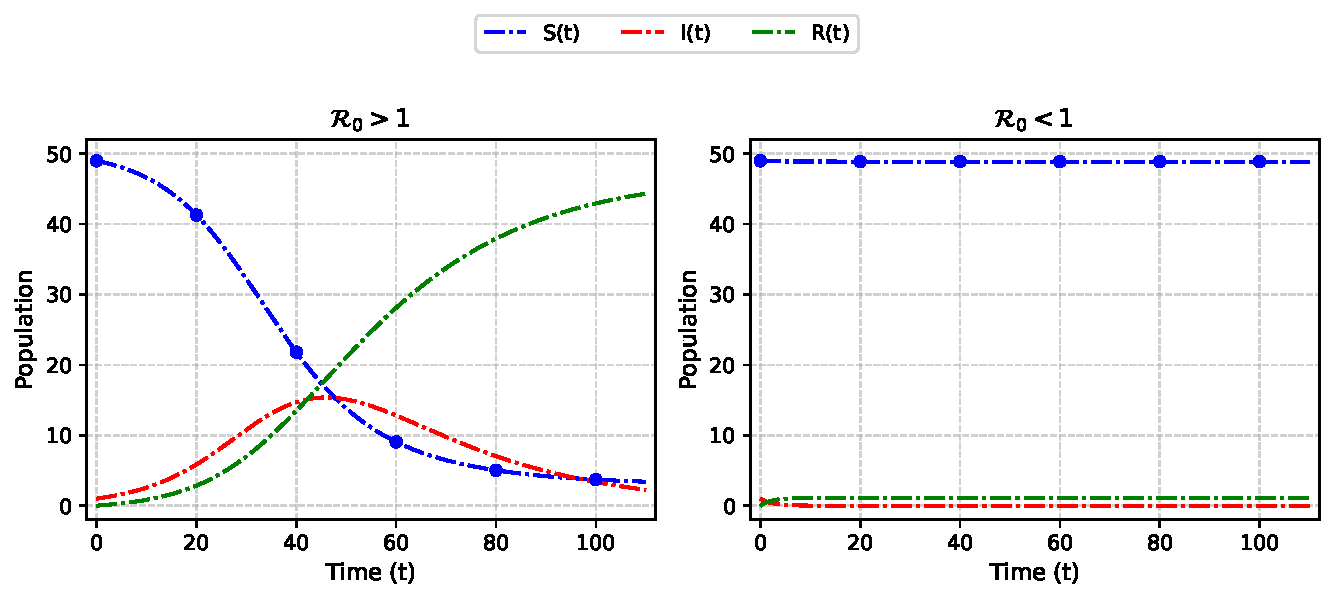
\includegraphics[width=\textwidth]{figures/sir_trajectories.pdf}
  \caption{Trajectories of the SIR model with $\mathcal{R}_0>1$ (Left) and $\mathcal{R}_0 < 1$ (Right). 
  Dash-dot lines denote the continuous simulation of susceptible ($S(t)$), infected ($I(t)$), and recovered ($R(t)$) populations.
  To strictly minimize approximation errors, the simulation is generated via a high-order numerical solver, specifically the explicit Runge-Kutta method of order 5(4)~\cite{dormand1980family}.
  Dots represent the partial and sparse observations sampled over the time interval $[0, 110]$ with a sparse time step of $\Delta t = 20$, which constitute the data available to our framework for parameter inference.
  The contrasting dynamics illustrate the bifurcation governed by $\mathcal{R}_0$:
  an epidemic outbreak regime on the left ($\beta=0.15, \gamma=0.05 \implies \mathcal{R}_0 =3.0$), characterized by a bell-shaped peak of $I(t)$ that induces a steep, sigmoidal drop in $S(t)$, versus a decay regime on the right ($\beta=0.05, \gamma=0.35 \implies \mathcal{R}_0 \approx 0.14$), where $I(t)$ decays monotonically, leaving $S(t)$ relatively flat and gradually decreasing.}
  \label{fig:sir_traj}
\end{figure}
% 흑백 프린트 하니까 구분이 잘 안 됨. 컬러맵 수정 필요

\subsection{Lotka-Volterra Model}
\label{subsec:lotka-volterra}

The Lotka-Volterra (LV) model is a periodic dynamical system describing the interaction between prey and predator populations~\cite{lotka1925elements, volterra1927fluctuations}. 
The state vector is $\mathbf{x}(t) = [x(t), y(t)]^\top$, where $x(t)$ and $y(t)$ represent the prey and predator populations, respectively. 
The system dynamics are governed by
\begin{equation}
\label{eq:lv}
    \dot{\mathbf{x}}(t) = f(\mathbf{x}(t), \theta) = 
    \begin{bmatrix}
        \alpha x(t) - \beta x(t)y(t) \\[6pt]
        \delta x(t)y(t) - \gamma y(t)
    \end{bmatrix},
    \quad t \in [0, T],
\end{equation}
where $x(t)>0$, $y(t)>0$ and the parameter vector is $\theta = [\alpha, \beta, \delta, \gamma]^\top \in \mathbb{R}^4_{>0}$. 
These parameters represent the prey birth rate $\alpha$, the predation rate $\beta$, the predator reproduction rate $\delta$, and the predator death rate $\gamma$.

The LV model provides a critical comparison to the SIR model not only in its oscillatory dynamics but also in its structural constraints. 
While the SIR model benefits from the linear population conservation ($I(t) \le \bar{N} - S(t)$) that strictly bounds the feasible region of the hidden state, the LV system lacks such trivial linear bounds. 
Instead, its trajectories are strictly confined to a level set of a nonlinear invariant manifold defined by the energy function:
\begin{equation}
\label{eq:lv_conserve}
    V(x,y) = \delta x - \gamma \ln x + \beta y - \alpha \ln y.
\end{equation}
Along any valid trajectory, this quantity remains constant $C>0$ such that $V(x(0), y(0)) \equiv C$.
Critically, this nonlinear constraint is explicitly coupled with the parameters $\theta$.
This implies that even if the prey $x(t)$ is observed, the feasible region for the hidden state $y(t)$ cannot be narrowed down without simultaneously identifying $\theta$. 
Consequently, parameter estimation and hidden state inference for the LV model formulate a fundamentally more ill-posed problem than for the SIR model.

Under the partial and sparse observation setting, we assume that only the prey population $x(t)$ is observable, that is, the observation function is defined as a projection $h(\mathbf{x}(t)) = x_\mathrm{obs}(t) = x(t)$.
A highly sparse observation regime is employed to evaluate the parameter estimation framework. 
Specifically, the observed data is restricted to a fixed time interval $t \in [0, 20]$ on a discrete grid of $N=10$ evenly spaced points, resulting in a coarse time step of $\Delta t \approx 2.22$.
To construct simulation datasets that capture the system's periodic nature without altering this fixed grid, we control the initial conditions based on the relative energy level $\Delta V = V(x(0), y(0)) - V(x^*, y^*)$, where $(x^*, y^*) = (\gamma/\delta, \alpha/\beta)$ is the equilibrium point. 
In practice, these initial conditions are generated via a rejection sampling scheme. 
Candidate coordinates $(x_0, y_0)$ are drawn uniformly from a bounded box surrounding the equilibrium point, and a candidate is accepted only if its relative energy strictly satisfies $C_{\min} \le \Delta V \le C_{\max}$. 
Here, the lower bound $C_{\min} > 0$ explicitly excludes trivial, near-linear harmonic oscillations, ensuring the dataset maintains a baseline level of nonlinearity. 
Conversely, the upper bound $C_{\max}$ mathematically guarantees that at least one full closed orbit is encompassed within $T=20$. 
Detailed specifications regarding the parameter distributions and exact boundary values for dataset generation are deferred to Section \ref{sec:experiments}.

This energy-based sampling strategy explicitly governs the difficulty of the inverse problem.
For small perturbations near the equilibrium, the system exhibits near-linear harmonic oscillations with a fundamental frequency $\omega_0 = \sqrt{\alpha\gamma}$. 
Under our parameter configuration, the corresponding minimum period is $T_0 \approx 7.85$, meaning the discrete grid ($\Delta t \approx 2.22$) places roughly 3.5 observation points per cycle. 
This sampling rate safely satisfies the \emph{Nyquist-Shannon sampling theorem}~\cite{shannon2006communication}, ensuring that the continuous dynamics can be adequately resolved.

However, as $\Delta V$ increases, the nonlinearities dominate, and the orbits degenerate into relaxation oscillations. 
In the time domain, these high-energy trajectories exhibit pronounced stiffness, characterized by extremely sharp, rapid transient spikes followed by slow recoveries. 
According to the Nyquist-Shannon sampling theorem, capturing such rapid transitions necessitates a substantially higher Nyquist frequency. 
Consequently, the fixed discrete grid falls critically short of this requirement, inducing severe temporal aliasing. 
This undersampling effectively obliterates the local gradient information during the peaks, meaning the true system dynamics cannot be recovered from local temporal differences alone. 
Thus, our framework is explicitly challenged to leverage the global nonlinear physical constraint \eqref{eq:lv_conserve} as an inductive bias, demonstrating its capacity to reconstruct the hidden state and parameters from the underlying topological geometry rather than highly aliased local transitions.

Figure \ref{fig:lv_traj} illustrates the core challenge of the LV model under this high-energy state.
While the continuous full state $\mathbf{x}(t)$ traces a closed orbit along the nonlinear manifold (Figure~\ref{fig:lv_traj}, Right), only the highly sparse and aliased observations $\left\{x_\mathrm{obs}(t_i)\right\}_{i=0}^{9}$ are available for inference (Figure~\ref{fig:lv_traj}, Left).
Notice how the fixed sampling grid severely misses the sharp nonlinear peaks, demonstrating the temporal aliasing phenomenon.
Thus, the underlying task demands the implicit reconstruction of this global nonlinear geometry solely from these sparse, localized observations.


\begin{figure}[t]
  \centering
  
  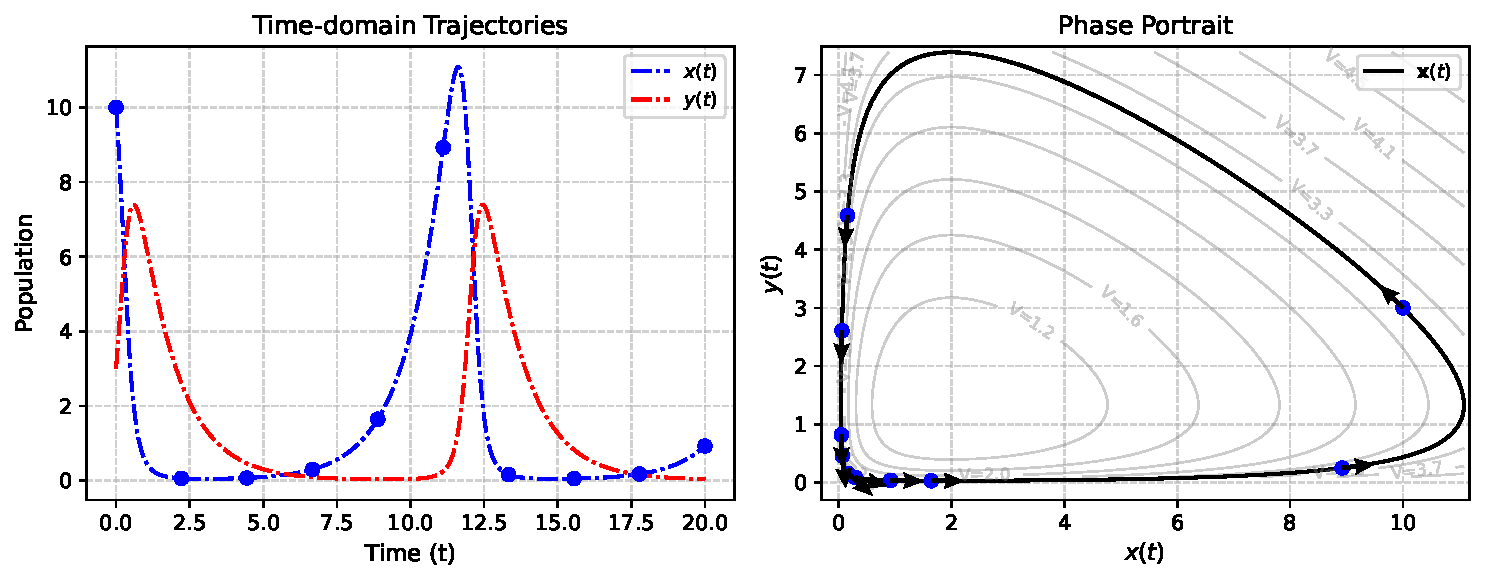
\includegraphics[width=\textwidth]{figures/lv_trajectories.pdf}
  \caption{Trajectories and phase portrait of the Lotka-Volterra model.  
    (Left) Time-domain trajectories of the observed prey $x(t)$ and hidden predator $y(t)$. 
    Dots indicate the sparse observations of $x(t)$, sampled at $N=10$ equally spaced points over the time interval $t \in [0, 20]$. 
(Right) Phase portrait in the $x-y$ plane. 
The continuous state evolution $\mathbf{x}(t)$ forms a closed orbit along the level set of the energy function $V(x,y)$ (background contours). 
The continuous trajectories were generated via the explicit Runge-Kutta method of order 5(4)~\cite{dormand1980family} with parameters $\alpha=0.8, \beta=0.6, \delta=0.4, \gamma=0.8$ and initial conditions $x(0)=10.0, y(0)=3.0$. 
This configuration yields a high energy level of $V(x(0), y(0)) \approx 3.08$, visually demonstrating how the discrete sampling grid fails to capture the sharp transient spikes.}
  \label{fig:lv_traj}
\end{figure}


\subsection{OGTT model}
\label{subsec:ogtt}

To be written....
% Section 4:
%\section{Feasibility: Identifiability and Observability Analysis}
\label{sec:identifiability}

Algorithmic convergence of the fixed-point iteration guarantees mathematical stability, but it does not ensure correct parameter recovery if the underlying inverse problem is structurally ill-posed. In this section, we analyze the structural identifiability of our benchmark systems using the nonlinear observability framework of Hermann and Krener \cite{hermann1977nonlinear}.

\subsection{Nonlinear Observability Framework}
We formulate parameter identifiability as a state observability problem by augmenting the state space. Let $\mathbf{x} \in \mathbb{R}^d$ be the system state and $\theta \in \mathbb{R}^p$ be the constant unknown parameters. We define the augmented state $\mathbf{z} = [\mathbf{x}^\top, \theta^\top]^\top \in \mathcal{M} \subseteq \mathbb{R}^{m}$, where $m = d+p$. The augmented dynamics and observation map are:
\begin{equation}
    \dot{\mathbf{z}} = F(\mathbf{z}) = \begin{bmatrix} f(\mathbf{x}, \theta) \\ \mathbf{0} \end{bmatrix}, \quad \mathbf{x}_{obs} = \tilde{h}(\mathbf{z}) = h(\mathbf{x}).
\end{equation}
Following Hermann and Krener, we construct the observability map $\Phi(\mathbf{z}): \mathcal{M} \to \mathbb{R}^{m \times d_{obs}}$ using successive Lie derivatives of the observation function $\tilde{h}$ along the vector field $F$:
\begin{equation}
    \Phi(\mathbf{z}) = \begin{bmatrix} \tilde{h}(\mathbf{z}) \\ L_{F} \tilde{h}(\mathbf{z}) \\ \vdots \\ L_{F}^{m-1} \tilde{h}(\mathbf{z}) \end{bmatrix},
\end{equation}
where $L_F \tilde{h}(\mathbf{z}) = \nabla_{\mathbf{z}} \tilde{h}(\mathbf{z}) \cdot F(\mathbf{z})$. 
The local observability matrix is defined as the Jacobian $\mathbf{O}(\mathbf{z}) := \nabla_{\mathbf{z}} \Phi(\mathbf{z})$. If $\mathbf{O}(\mathbf{z})$ has full rank $m$, the system satisfies the observability rank condition, meaning the observation map is locally a diffeomorphism, and the full augmented state $\mathbf{z}$ (including parameters $\theta$) can be uniquely reconstructed from the observations.

\subsection{SIR: Exact Observability via Lie Derivatives}
For the SIR compartmental model of epidemic dynamics~\cite{kermack1927contribution}, the recovered population $R$ is strictly determined by the conservation law ($N = S+I+R$). Thus, the effective augmented state is $\mathbf{z} = [S, I, \beta, \gamma]^\top \in \mathbb{R}^4$. Under the partial observation setting, only the susceptible population is observed, yielding $\tilde{h}(\mathbf{z}) = S$. 

We explicitly construct the $4 \times 4$ observability matrix by computing the sequence of Lie derivatives along the augmented vector field $F(\mathbf{z}) = [-\beta \frac{SI}{N}, \beta \frac{SI}{N} - \gamma I, 0, 0]^\top$. The first two gradient vectors are derived as:
\begin{align}
    \nabla_{\mathbf{z}} L_{F}^0 \tilde{h}(\mathbf{z}) &= [1, 0, 0, 0], \\
    \nabla_{\mathbf{z}} L_{F}^1 \tilde{h}(\mathbf{z}) &= \left[-\frac{\beta I}{N}, -\frac{\beta S}{N}, -\frac{SI}{N}, 0\right].
\end{align}
Continuing this process up to $L_F^3 \tilde{h}(\mathbf{z})$ systematically embeds the nonlinear interactions of $S, I, \beta$, and $\gamma$ into the rows of $\mathbf{O}(\mathbf{z})$. Evaluating the determinant of the resulting matrix confirms that $\text{rank } \mathbf{O}(\mathbf{z}) = 4$ for generic states $\mathbf{z}$. This direct algebraic calculation rigorously proves that the SIR system is structurally identifiable from $S(t)$ alone. The complete step-by-step derivation of the observability matrix is provided in Appendix \ref{app:obs-sir}.

\subsection{Lotka-Volterra: Unidentifiability via Symbolic Arithmetic}
For the Lotka--Volterra predator--prey system~\cite{lotka1925elements,volterra1927fluctuations}, the augmented state expands to dimension $m = 6$, given by $\mathbf{z} = [x, y, \alpha, \beta, \delta, \gamma]^\top$. The observation function isolates the prey population, $\tilde{h}(\mathbf{z}) = x$.

Constructing the corresponding $6 \times 6$ observability matrix $\mathbf{O}(\mathbf{z})$ requires evaluating up to the 5th-order Lie derivative ($L_F^5 \tilde{h}$). Due to the exponential growth of polynomial cross-terms, manual derivation becomes intractable. Therefore, we utilize symbolic algebraic computation (via SymPy) to generate the gradients and assemble $\mathbf{O}(\mathbf{z})$. The symbolic evaluation analytically confirms that:
\begin{equation}
    \text{rank } \mathbf{O}(\mathbf{z}) = 5 < 6.
\end{equation}
Because the algebraic rank is strictly less than the dimension of the augmented state space, the system is not locally observable from prey-only observations. As illustrated in Figure \ref{fig:lv_unidentifiable}, this rank deficiency implies the existence of distinct combinations of hidden predator trajectories and interaction parameters that map to the exact same prey trajectory $\mathbf{x}_{obs}(t)$. The SymPy code utilized for this exact algebraic derivation is included in Appendix \ref{app:obs-lv}.

\begin{figure}[htbp]
  \centering
  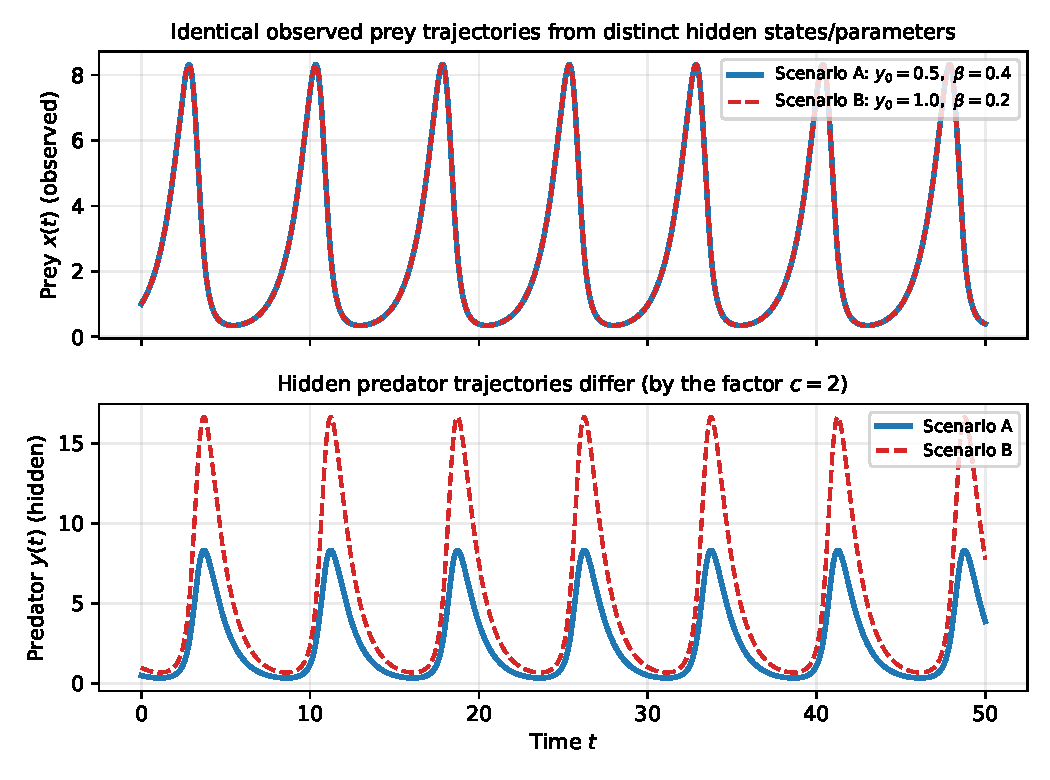
\includegraphics[width=0.82\textwidth]{figures/lv_nonident.pdf}
  %\framebox{\parbox{0.8\textwidth}{\centering
  %  \vspace{3cm}
  %  \textbf{} \\
  %  \small\textit{Identical prey observations $x(t)$ (top) from completely different hidden predator states $y(t)$ and parameter $\beta$ (bottom).}
  %  \vspace{3cm}
  %}}
  \caption{Structural unidentifiability in the Lotka-Volterra model. Scenario A ($x_0=1.0, y_0=0.5, \beta=0.4$) and Scenario B ($x_0=1.0, y_0=1.0, \beta=0.2$) produce identical observable trajectories for the prey $\mathbf{x}_{obs}(t)$ (top), despite originating from completely different hidden predator states and parameters (bottom). This algebraic indistinguishability proves that the full system cannot be identified from partial observations alone.}
  \label{fig:lv_unidentifiable}
\end{figure}

\subsection{OGTT: Jacobian Approximation and Theoretical Observability}
\label{subsec:ident-ogtt}
For the OGTT (oral glucose tolerance test) glucose--insulin minimal model~\cite{ha2025disposition}, the augmented state is
\begin{equation*}
\mathbf{z} = [G, I, N_5, N_6, S_I, \sigma]^\top \in \mathbb{R}^6, \qquad \mathbf{x}_{obs} = \tilde{h}(\mathbf{z}) = G .
\end{equation*}
Due to the high dimensionality and nested recurrences in the vector field, deriving $\mathbf{O}(\mathbf{z})$ even via symbolic computation is intractable.

Instead, we employ a Jacobian-based numerical approximation. The Taylor expansion of the observation $\mathbf{x}_{obs}(t)$ near $t=0$ can be expressed using Lie derivatives:
\begin{equation}
    \mathbf{x}_{obs}(t) = L_{F}^0 \tilde{h}(\mathbf{z}(0)) + t L_{F}^1 \tilde{h}(\mathbf{z}(0)) + \frac{t^2}{2!} L_{F}^2 \tilde{h}(\mathbf{z}(0)) + \dots
\end{equation}
Taking the gradient with respect to the initial augmented state $\mathbf{z}(0)$ and truncating at dimension $d=6$, the Jacobian $\mathbf{J} = \nabla_{\mathbf{z}(0)} \mathbf{x}_{obs}(\mathbf{t})$ evaluated at $T \ge 6$ discrete time points factors into:
\begin{equation}
    \mathbf{J} \approx \underbrace{\begin{bmatrix} 1 & t_1 & \dots & \frac{t_1^{d-1}}{(d-1)!} \\ \vdots & \vdots & \ddots & \vdots \\ 1 & t_T & \dots & \frac{t_T^{d-1}}{(d-1)!} \end{bmatrix}}_{\mathbf{T}} \underbrace{\begin{bmatrix} \nabla_{\mathbf{z}} L_{F}^0 \tilde{h}(\mathbf{z}(0)) \\ \vdots \\ \nabla_{\mathbf{z}} L_{F}^{d-1} \tilde{h}(\mathbf{z}(0)) \end{bmatrix}}_{\mathbf{O}(\mathbf{z}(0))}.
\end{equation}
Since the Vandermonde matrix $\mathbf{T}$ has full column rank for distinct time points, $\text{rank}(\mathbf{J}) = \text{rank}(\mathbf{O}(\mathbf{z}))$. We estimate $\text{rank}(\mathbf{J})$ using finite differences and Singular Value Decomposition (SVD), carefully normalizing the scale of each variable. 

The SVD yields six strictly positive singular values ($\varsigma_1 \approx 1.2\times 10^{2} \dots \varsigma_6 \approx 1.5\times 10^{-3}$; Figure~\ref{fig:ogtt_sensitivity}, left), all well above machine zero (we write $\varsigma$ for singular values to avoid collision with the parameter $\sigma$). This confirms that $\text{rank}(\mathbf{O}) = 6$. Theoretically, under idealized conditions with sufficient time steps and high-order derivative information, the OGTT system is structurally identifiable from glucose alone.

\subsection{Bridging Theory and Practice: The Ill-Conditioning of OGTT}
While theoretically identifiable, the SVD spectrum reveals a critical practical challenge. The singular values span roughly five orders of magnitude, indicating that the Jacobian $\mathbf{J}$ is severely ill-conditioned.

\begin{figure}[htbp]
  \centering
  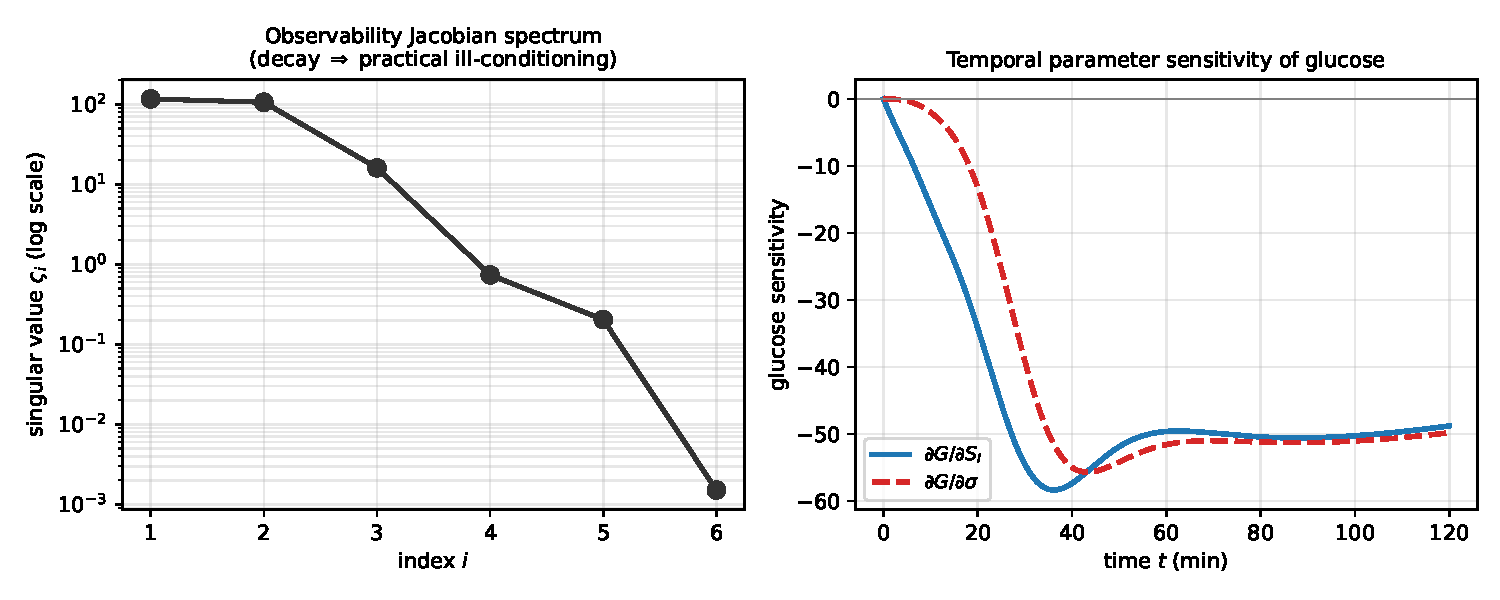
\includegraphics[width=0.92\textwidth]{figures/ogtt_illcond.pdf}
  %\framebox{\parbox{0.8\textwidth}{\centering
  %  \vspace{3cm}
  %  \textbf{} \\
  %  \small\textit{(Left) Singular value spectrum showing steep decay. (Right) Normalized sensitivity dynamics of $S_I$ and $\sigma$ over time.}
  %  \vspace{3cm}
  %}}
  \caption{Ill-conditioning and parameter sensitivity in the OGTT model. (Left) The singular values of the Jacobian decay rapidly, indicating practical unidentifiability despite theoretical full rank. (Right) The temporal sensitivity of glucose to $S_I$ and $\sigma$. Early dynamics ($<30$ min) are dominated by $S_I$, while later dynamics entangle the effects of both parameters.}
  \label{fig:ogtt_sensitivity}
\end{figure}

This ill-conditioning manifests temporally. As shown in Figure \ref{fig:ogtt_sensitivity} (Right), the sensitivity of glucose to insulin sensitivity ($\partial G / \partial S_I$) rises first, becoming strongest within the first $30$--$40$ minutes. The influence of $\beta$-cell function ($\partial G / \partial \sigma$) instead builds up more slowly, along a sigmoid-like profile. In the later stages, the two sensitivities become comparable and the coupled influence of both parameters dictates the glucose trajectory. Under a uniform 30-minute sampling grid without continuous flow information, the neural network struggles to disentangle these intertwined sensitivities. This translates the theoretically full-rank system into a practically unidentifiable regime, severely limiting the precise joint recovery of $(S_I, \sigma)$ and paving the way for the regression-to-mean phenomenon.


% Section 5:
\section{Method: Iteration of Two Networks for Parameter Estimation}
\label{sec:method}

This section presents an iterative neural network framework for parameter estimation from partial and sparse observations.
To motivate our approach, consider the forward mapping from the parameter to the partial observations.
As illustrated in Figure~\ref{fig:motive}, this mapping consists of two distinct steps:
integrating the governing ODE $\dot{\mathbf{x}}=f(\mathbf{x};\theta)$ to obtain the full state $\mathbf{x} = \left[\mathbf{x}_\mathrm{obs}, \mathbf{x}_\mathrm{hid}\right]^\top$, and applying a non-injective projection $h(\mathbf{x})=\mathbf{x}_\mathrm{obs}$ to obtain the partial observation.

A direct regression from partial observations to parameters bypasses this two-step structure and never forms an explicit estimate of the hidden state $\mathbf{x}_\mathrm{hid}$. Because different hidden states and parameters can generate the same partial observation, it is tempting to conclude that ignoring $\mathbf{x}_\mathrm{hid}$ must discard information and that a method reconstructing it should do better. This intuition motivates the decoupled design developed below; we return to it critically in Section~\ref{sec:correctness}, where we show that at inference the reconstructed hidden state is itself a function of the observation and therefore confers no such information advantage.

Instead of a direct map, we invert the forward mapping step-by-step.
We decompose the inverse problem into two stages:
(i) inferring the full state $\mathbf{x}$ from the partial observation $\mathbf{x}_\mathrm{obs}$, and 
(ii) estimating the parameter $\theta$ from the full state $\mathbf{x}=[\mathbf{x}_\mathrm{obs}, \mathbf{x}_\mathrm{hid}]^\top$.
However, this decomposition introduces a circular dependency.
Estimating the full state $\mathbf{x}$ requires the parameter $\theta$ to resolve the non-injectivity of the projection $h$, and estimating the parameter $\theta$ requires the full state $\mathbf{x}$.

\begin{figure}[htbp]
    \centering
    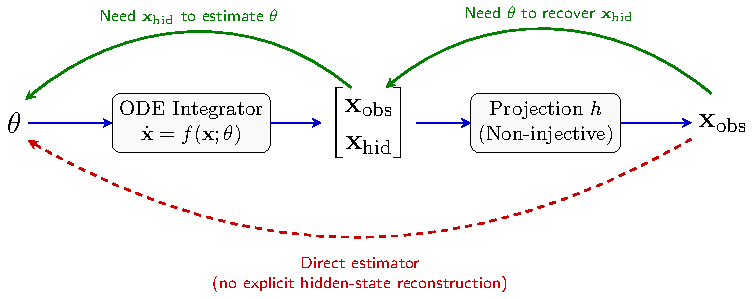
\includegraphics[width=0.8\linewidth]{figures/motive_fig.pdf}
    \caption{Illustration of the forward mapping and the inherent circular dependency in the inverse problem. 
    The forward process generates the full state via an ODE integrator, followed by a non-injective projection $h$ that yields the partial observation $\mathbf{x}_{\text{obs}}$.
    A direct estimator (red dashed arrow) maps the observation to the parameter without forming the hidden state.
    Inverting this process step-by-step requires resolving a circular dependency: estimating the parameter $\theta$ requires the hidden state $\mathbf{x}_{\text{hid}}$ (left green arrow), while recovering $\mathbf{x}_{\text{hid}}$ necessitates prior knowledge of $\theta$ (right green arrow).}
    \label{fig:motive}
\end{figure}

To resolve this dependency, we propose the iterative neural network framework shown in Figure~\ref{fig:method_overview}.
We introduce two neural networks designed to mimic the step-by-step inversion by acting as conditional estimators.
The hidden-state estimator $H_\phi:(\mathbf{x}_\mathrm{obs},\theta)\mapsto \mathbf{x}_\mathrm{hid}$ estimates the hidden state $\mathbf{x}_\mathrm{hid}$ from the observation $\mathbf{x}_\mathrm{obs}$ conditioned on a specific parameter guess $\theta$.
Subsequently, the parameter estimator $P_\psi:(\mathbf{x}_\mathrm{obs}, \mathbf{x}_\mathrm{hid})\mapsto \theta$ refines the parameter guess using the completed trajectory.
These networks are trained independently using decoupled supervised learning to prevent error accumulation, as illustrated in Figure~\ref{fig:method_train}. 
During inference, they are coupled to form a fixed-point iteration operator, continuously updating the parameter estimate as follows:
\begin{equation}
    \hat\theta^{(k+1)}=\mathcal{T}(\hat\theta^{(k)};\mathbf{x}_\mathrm{obs}) := P_\psi(\mathbf{x}_\mathrm{obs},H_\phi(\mathbf{x}_\mathrm{obs},\hat\theta^{(k)})).
\end{equation}
By alternating between the hidden state and parameter updates, the estimate converges to a network-consistent fixed point $\theta^*$ that resolves the circular dependency (whether this network-consistent point is also observation-consistent is the subject of Section~\ref{sec:correctness}).
The remainder of this section details the data representation, the iteration operator $\mathcal{T}$, and the training and inference algorithms.

% figure 위치가 필요한 기호들이 나오기 전에 있어서 약간 이해하기가 곤란한 듯.

\subsection{Data Representation}
\label{subsec:data_gen}

To train the estimators via supervised learning, we generate a synthetic dataset by simulating the dynamics.
We sample parameters $\theta$ and initial conditions $\mathbf{x}(t_0)$ from a predefined training distribution $\mathcal{P}_\mathrm{train}$, solve the initial value problem for the ODE~\eqref{eq:ode} on $[0, T]$ via a numerical solver, and record the states at the sampling times $t_0, \ldots, t_{N}$. 
This procedure yields an i.i.d. dataset $\mathcal{D}$ of $M$ trajectories:

\begin{equation}
\label{eq:training-samples}
\mathcal{D}:=\left\{(\mathbf{x}_{\mathrm{obs}}^{(m)},\mathbf{x}_{\mathrm{hid}}^{(m)},\theta^{(m)})\right\}_{m=1}^M,
\end{equation}
where $\mathbf{x}_{\mathrm{obs}}^{(m)}$ and $\mathbf{x}_{\mathrm{hid}}^{(m)}$ are the flattened vectors defined in Section~\ref{sec:problem}.
Prior to training, these vectors are scaled via a dataset-level normalization scheme (fit on the training split only) to ensure numerical stability.

\subsection{Fixed-Point Iteration Operator}

Given an observation $\mathbf{x}_\mathrm{obs}$, our objective is to accurately infer the corresponding system parameter $\theta$ in accordance with the data generation process as illustrated in Figure~\ref{fig:motive}.
We formulate this parameter estimation as finding a fixed-point of a discrete dynamical system defined by an iterative operator. 
To achieve this, we decompose the estimation problem into two subtasks and construct mappings to perform each.

The first mapping is the hidden-state estimator $H_\phi$, which solves a full state recovery task:
\begin{equation}
    \label{eq:H-map}
        H_\phi:\mathbb{R}^{(N+1)d_{\mathrm{obs}}}\times \mathbb{R}^{p}\to \mathbb{R}^{(N+1)d_{\mathrm{hid}}},
            \quad
        (\mathbf{x}_\mathrm{obs},\theta) \mapsto \hat{\mathbf{x}}_{\mathrm{hid}}.
\end{equation}
This mapping takes the observation $\mathbf{x}_\mathrm{obs}$ and a specific parameter guess $\theta$ as inputs to estimate the corresponding hidden state $\hat{\mathbf{x}}_{\mathrm{hid}}$.
Conditioning on $\theta$ supplies $H_\phi$ with side information that the projection $h$ discards, so that it can estimate a full state trajectory $\mathbf{x}=[\mathbf{x}_\mathrm{obs}, \hat{\mathbf{x}}_\mathrm{hid}]^\top$ consistent with the underlying dynamics; we emphasize that this addresses the non-injectivity of $h$ only relative to the supplied guess, and does not by itself resolve the non-identifiability of $\theta$ from $\mathbf{x}_\mathrm{obs}$ (Section~\ref{sec:correctness}).

The second mapping is the parameter estimator $P_\psi$, which solves a parameter estimation task from the full-state:
\begin{equation}
\label{eq:P-map}
    P_\psi:\mathbb{R}^{(N+1)d_{\mathrm{obs}}}\times \mathbb{R}^{(N+1)d_{\mathrm{hid}}}\to \mathbb{R}^{p},
    \quad
    (\mathbf{x}_\mathrm{obs},\mathbf{x}_{\mathrm{hid}}) \mapsto \hat{\theta}.
\end{equation}
This mapping deduces the parameter vector from the reconstructed full-state trajectory.

We implement both mappings as multi-layer perceptrons (MLPs) parameterized by $\phi$ and $\psi$, respectively; the choice of a flexible, expressive hypothesis class is what makes each conditional mapping learnable from data.

By composing these  two networks, we define the iteration operator $\mathcal{T}(\cdot ;\mathbf{x}_\mathrm{obs}):\Theta \to \Theta$, given by
\begin{equation}
    \label{eqn:iter_oper}
    \mathcal{T}(\theta;  \mathbf{x}_\mathrm{obs}) := P_\psi(\mathbf{x}_\mathrm{obs}, H_\phi(\mathbf{x}_\mathrm{obs}, \theta)).
\end{equation}
This composite operator acts as a discrete dynamical system in parameter space.
We refer to $\mathcal{T}$ as the \emph{fixed-point iteration operator}.
Finding a fixed point $\theta^*$ such that $\theta^*=\mathcal{T}(\theta^*;\mathbf{x}_\mathrm{obs})$ provides a mechanism to resolve the cyclic dependency between two subtasks.

\begin{figure}[htbp]
    \centering
    
    % (a) Training 
    % 가로 배치를 위해 폭을 텍스트 폭의 48%로 설정
    \subfloat[Supervised training via teacher forcing\label{fig:method_train}]{
        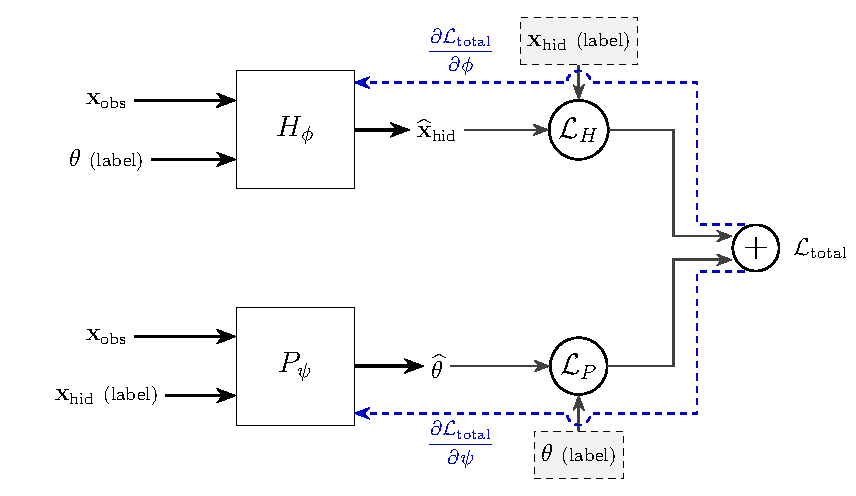
\includegraphics[width=0.50\textwidth]{figures/fig_training.pdf}
    }
    \hfill % 두 그림 사이의 가로 여백
    % (b) Inference
    \subfloat[Inference via alternating iteration\label{fig:method_infer}]{
        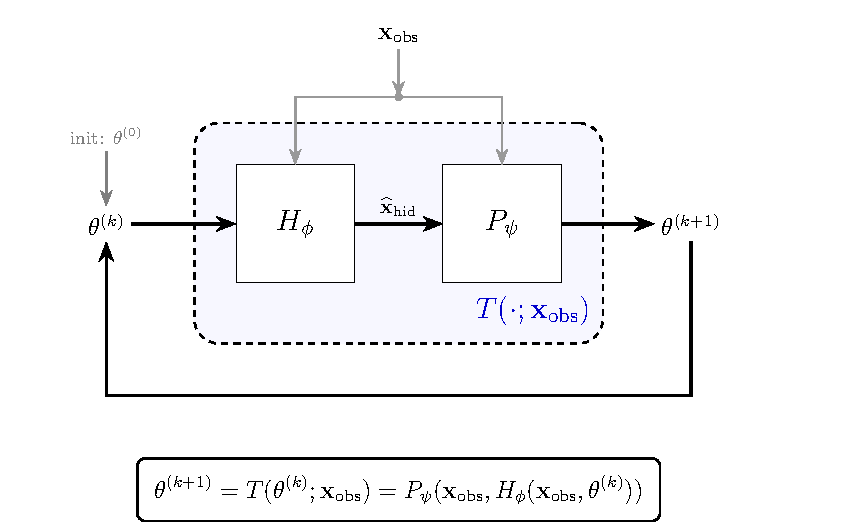
\includegraphics[width=0.45\textwidth]{figures/fig_infer.pdf}
    }
    
    \caption{Overview of the proposed fixed-point iteration networks. 
    The training and inference pipelines are connected but structurally distinct.
    \textbf{(a)} During training, the hidden-state estimator $H_\phi$ and the parameter estimator $P_\psi$ are decoupled. 
    Ground-truth values are provided to optimize $\mathcal{L}_H$ and $\mathcal{L}_P$ independently. 
    \textbf{(b)} At inference, given sparse observations $\mathbf{x}_\mathrm{obs}$, the networks are coupled to define a fixed-point update operator $\mathcal{T}(\cdot; \mathbf{x}_\mathrm{obs})$.}
    \label{fig:method_overview}
\end{figure}

\subsection{Decoupled Supervised Training}
\label{subsec:training}

We train the networks $H_\phi$ and $P_\psi$ in a supervised manner using the synthetic dataset $\mathcal{D}$ generated in Section~\ref{subsec:data_gen}. 
As illustrated in Figure~\ref{fig:method_train}, we train the two networks independently without cyclic dependency to prevent error accumulation. 
This decoupled approach is conceptually analogous to \emph{teacher forcing} \cite{williams1989learning}. 
During inference, $H_\phi$ must rely on a previously estimated parameter $\hat{\theta}^{(k)}$ as its conditional input, and $P_\psi$ must rely on the estimated hidden state $\hat{\mathbf{x}}_{\mathrm{hid}}^{(k+1)}$.
If trained jointly in this coupled manner, early estimation errors would propagate and amplify across the networks.
In our teacher-forced training, we break this cycle by substituting the unavailable inference-phase estimates with exact ground-truth values. 
Specifically, we provide the true parameter $\theta^\mathrm{true}$ as the conditional input to $H_\phi$ (targeting the true $\mathbf{x}_{\mathrm{hid}}^\mathrm{true}$), and provide the true state $\mathbf{x}_{\mathrm{hid}}^\mathrm{true}$ as the conditional input to $P_\psi$ (targeting the true $\theta^\mathrm{true}$).

Given a training sample $(\mathbf{x}_{\mathrm{obs}}, \mathbf{x}_{\mathrm{hid}}^\mathrm{true}, \theta^\mathrm{true}) \sim \mathcal{D}$, we optimize the network parameters $\phi$ and $\psi$ by minimizing their respective mean squared error (MSE) loss functions:
\begin{align}
    \mathcal{L}_H(\phi) &:= \mathbb{E}_{\mathcal{D}} \left[ \left\| H_\phi(\mathbf{x}_{\mathrm{obs}}, \theta^\mathrm{true}) - \mathbf{x}_{\mathrm{hid}}^\mathrm{true} \right\|_2^2 \right], \label{eq:loss_h} \\
    \mathcal{L}_P(\psi) &:= \mathbb{E}_{\mathcal{D}} \left[ \left\| P_\psi(\mathbf{x}_{\mathrm{obs}}, \mathbf{x}_{\mathrm{hid}}^\mathrm{true}) - \theta^\mathrm{true} \right\|_2^2 \right]. \label{eq:loss_p}
\end{align}

Because the two networks do not feed their outputs to one another during training, their computational graphs are strictly disconnected. 
Consequently, when optimizing the total loss $\mathcal{L}_{\mathrm{total}} := \mathcal{L}_H(\phi) + \mathcal{L}_P(\psi)$ via stochastic gradient descent (SGD), the parameter updates are completely decoupled. 
As depicted in Figure~\ref{fig:method_train}, the gradients of the total loss reduce to the partial derivatives with respect to each network's parameters:
\begin{equation}
    \frac{\partial \mathcal{L}_{\mathrm{total}}}{\partial \phi} = \frac{\partial \mathcal{L}_H}{\partial \phi}, \qquad \frac{\partial \mathcal{L}_{\mathrm{total}}}{\partial \psi} = \frac{\partial \mathcal{L}_P}{\partial \psi}.
\end{equation}
These gradients are computed and applied independently without backpropagating errors across the networks. 

This teacher-forced protocol \emph{targets} an operator that preserves the ground truth,
\begin{equation*}
\mathcal{T}(\theta^\mathrm{true}; \mathbf{x}_{\mathrm{obs}}) \approx \theta^\mathrm{true}.
\end{equation*}
Whether the resulting fixed point actually coincides with the ground truth is a separate question, which we take up in Section~\ref{sec:correctness}: there we show that this target is in general unreachable under observational ambiguity, that the fixed point is bounded by the conditional mean, and that under non-identifiability the conditional mean is displaced off the solution fiber.

\subsection{Coupled Inference via Fixed-Point Iteration}
\label{subsec:inference}

Although training is strictly decoupled, inference requires coupling the two networks to form the fixed-point iteration operator $\mathcal{T}$, as illustrated in Figure~\ref{fig:method_infer}. At inference time, only the sparse and partial observation $\mathbf{x}_{\mathrm{obs}}$ is available; the ground-truth parameter and hidden states are completely unknown.

Starting from an initial parameter guess $\hat{\theta}^{(0)}$, we sequentially apply the alternating updates between the hidden-state estimator and the parameter estimator. The overall inference procedure is summarized in Algorithm~\ref{alg:inference}. 

\begin{algorithm}[t]
\caption{Fixed-step iterative inference for parameter estimation}
\label{alg:inference}
\begin{algorithmic}[1]
    \REQUIRE observed samples $\mathbf{x}_\mathrm{obs}=[x_{\mathrm{obs}}(t_0),\ldots,x_{\mathrm{obs}}(t_{N})]^\top$ ($N+1$ times);
    trained networks $H_\phi,P_\psi$; 
    number of iterations $K$
    %\STATE form $\tilde{\mathbf{x}}_{\mathrm{obs}}=\mathrm{vec}(\tilde{x}_{\mathrm{obs},0},\ldots,\tilde{x}_{\mathrm{obs},N-1})$
    %\STATE approximate the derivative features $\widehat{\dot{\mathbf{x}}}_{\mathrm{obs}}$ from $\mathbf{x}_\mathrm{obs}$ via spline interpolation
    %\STATE set $\mathbf{x}_\mathrm{obs}=\left[\mathbf{x}_{\mathrm{obs}},\widehat{\dot{\mathbf{x}}}_{\mathrm{obs}}\right]^\top$
    \STATE initialize $\hat{\theta}^{(0)}$ (e.g., centered at the dataset mean)
    \FOR{$k=0,1,\ldots,K-1$}
        \STATE $\widehat{\mathbf{x}}_{\mathrm{hid}}^{(k+1)} \gets H_\phi(\mathbf{x}_\mathrm{obs},\widehat{\theta}^{(k)})$
        \STATE $\widehat{\theta}^{(k+1)} \gets P_\psi(\mathbf{x}_\mathrm{obs},\widehat{\mathbf{x}}_{\mathrm{hid}}^{(k+1)})$
    \ENDFOR
    \RETURN $\widehat{\theta}^{(K)}$
\end{algorithmic}
\end{algorithm}

The iterative process defined in Algorithm~\ref{alg:inference} is mathematically equivalent to computing the orbit of the discrete dynamical system $\hat{\theta}^{(k+1)} = \mathcal{T}(\hat{\theta}^{(k)}; \mathbf{x}_{\mathrm{obs}})$. For this iteration to be stable and independent of the initial guess, the operator $\mathcal{T}(\cdot; \mathbf{x}_{\mathrm{obs}})$ must be a contraction mapping. We establish sufficient conditions for this contractivity in Section~\ref{sec:convergence}, showing that enforcing appropriate Lipschitz constraints on $H_\phi$ and $P_\psi$ guarantees global geometric convergence to a unique fixed point $\theta^*(\mathbf{x}_{\mathrm{obs}})$. Because of this exponential convergence rate, a very small number of iterations (e.g., $K = 1$ to $10$) typically suffices in practice to reach the fixed point.


% Section 6:
%6.1 iteration을 (\theta^{(k+1)} = T(\theta^{(k)})) 형태의 연산자로 정리
%6.2 (T)의 Lipschitz bound를 (H_\phi, P_\psi)의 Lipschitz 상수로 상계
%6.3 spectral normalization이 이를 어떻게 보장하는지(정리/조건)
%6.4 Theorem: unique fixed point + exponential convergence
%6.5 Corollary: K=10 고정이 충분한 이유(오차 bound로 연결 가능)

\section{Theory 1: Convergence}
\label{sec:convergence}

In this section we analyze the iteration operator
$\theta^{(k+1)} = \mathcal{T}(\theta^{(k)};\mathbf{x}_\mathrm{obs})$
introduced in \ref{sec:method}.
The introduction of the iteration raises a critical theoretical questions:

\emph{Convergence: Does this iteration process stably converge to a unique fixed point?}
\emph{Sensitivity: Is it sensitive to the initial guess $\theta^{(0)}$?}

In this section, we prove that by enforcing strict Lipschitz bounds on two neural networks $H_\phi$ and $P_\psi$, the composite operator $\mathcal{T}$ becomes a global contraction mapping, guaranteeing exponential convergence to a unique fixed point $\theta^*$ from any arbitrary initialization.

\subsection{Preliminaries: contraction mappings and Banach's theorem}
\label{subsec:banach}

Let $(\Theta,\|\cdot\|_2)$ be a complete metric space.
\footnote{In practice, $\Theta$ is taken as a closed subset of $\mathbb{R}^p$ in normalized coordinates.}
A map $\mathcal{T}:\Theta\to\Theta$ is a \textit{contraction} if there exists $K\in[0,1)$ such that

\begin{equation}
\label{eq:contraction-def}
    \lVert \mathcal{T}(\theta_a)-\mathcal{T}(\theta_b)\|_2 \le K\|\theta_a-\theta_b\rVert_2,
    \qquad \forall\,\theta_a,\theta_b\in\Theta.
\end{equation}

By \emph{Banach's fixed-point theorem}, a contraction has a unique fixed point $\theta^*$ and the iteration
$\theta^{(k+1)}=\mathcal{T}(\theta^{(k)})$ converges to $\theta^*$ for any initialization. 
Moreover, the convergence is geometric:

\begin{equation}
\label{eq:geom-rate}
    \|\theta^{(k)}-\theta^*\|_2 \le K^k\|\theta^{(0)}-\theta^*\|_2.
\end{equation}

\subsection{A Sufficient Condition for Contractivity of $\mathcal{T}$}
\label{subsec:contractivity}

Recall that our update operator is the composition:

\begin{equation}
\label{eq:T-repeat}
    \mathcal{T}(\theta;\mathbf{x}_\mathrm{obs}) = P_\psi\big(\mathbf{x}_\mathrm{obs}, H_\phi(\mathbf{x}_\mathrm{obs},\theta)\big).
\end{equation}

We provide a simple sufficient condition for \eqref{eq:contraction-def} in terms of Lipschitz constants of the two networks.

\begin{assumption}[Lipschitz continuity of the learned maps]
\label{ass:lipschitz}
    For each fixed input $\mathbf{x}_\mathrm{obs}$, the hidden-state estimator $H_\phi$ is Lipschitz in $\theta$:
    there exists $\mathrm{Lip}_H\ge0$ such that
    $$
    \lVert H_\phi(\mathbf{x}_\mathrm{obs},\theta_a)-H_\phi(\mathbf{x}_\mathrm{obs},\theta_b)\rVert_2 \le 
    \mathrm{Lip}_H\|\theta_a-\theta_b\|_2,
    \qquad \forall\,\theta_a,\theta_b\in\Theta.
    $$
    Moreover, the parameter estimator $P_\psi$ is Lipschitz in its hidden-state input:
    there exists $\mathrm{Lip}_P\ge0$ such that for all $\mathbf{z}_a,\mathbf{z}_b$ in the range of $H_\phi(\mathbf{x}_\mathrm{obs},\cdot)$,
    $$
    \lVert P_\psi(\mathbf{x}_\mathrm{obs},\mathbf{z}_a)-P_\psi(\mathbf{x}_\mathrm{obs},\mathbf{z}_b)\|_2 \le \mathrm{Lip}_P\|\mathbf{z}_a-\mathbf{z}_b\|_2.
    $$
\end{assumption}

\begin{theorem}[Contractivity of the Iterative Operator]
\label{thm:contraction}
    Under Assumption~\ref{ass:lipschitz}, the update operator $\mathcal{T}(\cdot;\mathbf{x}_\mathrm{obs})$ is Lipschitz with constant at most $\mathrm{Lip}_\mathcal{T}:=\mathrm{Lip}_P\mathrm{Lip}_H$:
    $$
    \|T(\theta_a;\mathbf{x}_\mathrm{obs})-T(\theta_b;\mathbf{x}_\mathrm{obs})\|_2 \le \mathrm{Lip}_P\mathrm{Lip}_H \|\theta_a-\theta_b\|_2,
    \qquad \forall\,\theta_a,\theta_b\in\Theta.
    $$
    In particular, if $\mathrm{Lip}_P\mathrm{Lip}_H<1$, then $\mathcal{T}(\cdot;\mathbf{x}_\mathrm{obs})$ is a contraction on $(\Theta,\|\cdot\|_2)$ and hence has a unique fixed point
    $\theta^*(\mathbf{x}_\mathrm{obs})$.
    Moreover, for any initialization $\theta^{(0)}\in\Theta$, the iteration $\theta^{(k+1)}=\mathcal{T}(\theta^{(k)};\mathbf{x}_\mathrm{obs})$ converges to
    $\theta^*(\mathbf{x}_\mathrm{obs})$ and satisfies the geometric rate bound \eqref{eq:geom-rate} with $\mathrm{Lip}_\mathcal{T}$.
\end{theorem}

\begin{proof}
    Fix $\mathbf{x}_\mathrm{obs}$ and let $\theta_a,\theta_b\in\Theta$.
    By \eqref{eq:T-repeat} and the Lipschitz property of $P_\psi$ in its second argument,
    \begin{align*}
        \lVert \mathcal{T}(\theta_a;\mathbf{x}_\mathrm{obs})-\mathcal{T}(\theta_b;\mathbf{x}_\mathrm{obs})\rVert_2
    &=
    \lVert P_\psi(\mathbf{x}_\mathrm{obs},H_\phi(\mathbf{x}_\mathrm{obs},\theta_a)) - P_\psi(\mathbf{x}_\mathrm{obs},H_\phi(\mathbf{x}_\mathrm{obs},\theta_b))\rVert_2
    \\
    &\le
    \mathrm{Lip}_P\lVert H_\phi(\mathbf{x}_\mathrm{obs},\theta_a)-H_\phi(\mathbf{x}_\mathrm{obs},\theta_b)\rVert_2.
    \end{align*}
    
    Applying the Lipschitz property of $H_\phi$ in $\theta$ yields
    $$
    \|\mathcal{T}(\theta_a;\mathbf{x}_\mathrm{obs})-\mathcal{T}(\theta_b;\mathbf{x}_\mathrm{obs})\|_2 \le \mathrm{Lip}_P\mathrm{Lip}_H\|\theta_a-\theta_b\|_2.
    $$
    Since $\mathrm{Lip}_\mathcal{T}=\mathrm{Lip}_P\mathrm{Lip}_H<1$, then $\mathcal{T}(\cdot;\mathbf{x}_\mathrm{obs})$ is a contraction and the remaining claims follow from Banach's fixed-point theorem.
\end{proof}

\subsection{Enforcing Lipschitz bounds via spectral normalization}
\label{subsec:sn}

Assumption~\ref{ass:lipschitz} can be promoted in practice by controlling the operator norms of the linear layers.
For a linear map $x\mapsto Wx$, its $\ell_2$-Lipschitz constant equals the spectral norm $\|W\|_2$.
Spectral normalization rescales each weight matrix $W$ by an estimate of $\|W\|_2$ so that the resulting layer has a prescribed operator-norm bound,
typically close to~$1$.
This idea was popularized in the deep learning literature as a training-stabilization technique. \cite{miyato2018spectralnormalizationgenerativeadversarial}

For a feed-forward network composed of linear layers and pointwise nonlinearities with Lipschitz constant at most~$1$ (e.g., $\tanh$),
one obtains a simple upper bound on the network's Lipschitz constant by multiplying the spectral norms of the weight matrices.
Consequently, by applying spectral normalization layerwise (and leaving a small margin for strict inequality),
we can ensure $\mathrm{Lip}_H$ and $\mathrm{Lip}_P$ are bounded and achieve $\mathrm{Lip}_P\mathrm{Lip}_H<1$.
Further implementation details are provided in the supplementary material.


Section~\ref{subsec:exp-convergence} verifies this empirically: without spectral normalization the
measured composite Lipschitz constant exceeds one and the iteration fails to contract, whereas across a
range of margins that keep $\mathrm{Lip}_\mathcal{T}<1$ the iteration converges as predicted.

\subsection{Implications for the number of inference steps}
\label{subsec:Ksteps}

Theorem~\ref{thm:contraction} yields a direct justification for using a small, fixed number of inference steps.
If $\mathcal{T}(\cdot;\mathbf{x}_\mathrm{obs})$ is a contraction with constant $K<1$, then after $k$ iterations,
$$
\lVert\theta^{(k)}-\theta^*(\mathbf{x}_\mathrm{obs})\rVert_2 \le K^k\lVert\theta^{(0)}-\theta^*(\mathbf{x}_\mathrm{obs})\rVert_2,
$$
so the error decreases exponentially in $k$.
This explains why in practice a small number of iterations (e.g., $K=10$) suffices, and why often $1$--$2$ iterations already yield a stable estimate.


% Section 7 (Correctness & statistical limitation; includes off-fiber sharpening):
\section{Theory 2: Correctness and Statistical Limitations}
\label{sec:correctness}

Theorem~\ref{thm:contraction} establishes that the iteration $\theta^{(k+1)} = \mathcal{T}(\theta^{(k)}; \mathbf{x}_\mathrm{obs})$ converges to a unique fixed point $\theta^*(\mathbf{x}_\mathrm{obs})$ from any initialization, but convergence says nothing about \emph{what} that fixed point is. This section characterizes it, and the conclusion is a characterization rather than a correctness guarantee. We establish four facts. First, contractivity and observational ambiguity are structurally \emph{incompatible}: a strict contraction cannot keep two distinct admissible parameters as zero-residual fixed points, so preserving the whole teacher-forced target is unreachable on a non-identifiable fiber (Section~\ref{subsec:incompat}). Second, because the fixed point is a deterministic function of $\mathbf{x}_\mathrm{obs}$, it cannot be more accurate than the conditional mean --- the Bayes performance ceiling under squared loss faced already by a plain direct regressor, which reconstructing the hidden state does \emph{not} circumvent (Section~\ref{subsec:ceiling}). Third, among all contractions the one that minimizes the idealized one-step risk has that conditional mean as its fixed point (Section~\ref{subsec:collapse}); we are careful to separate this idealized objective from the decoupled loss actually optimized in training. Fourth, whether that Bayes-optimal point is itself observation-consistent depends on the \emph{coordinate} in which the squared loss is taken: for a curved fiber the conditional mean lies off it, but a reparameterization that straightens the fiber --- logarithms for a product degeneracy --- keeps the conditional mean on the fiber (Section~\ref{subsec:off_fiber}). The overall picture is that the decoupled fixed-point estimator is a stable, convergent procedure whose accuracy is bounded by the conditional mean in the loss coordinate, and whose reconstruction of the hidden state confers no \emph{information-theoretic} advantage over an estimator based on the observation alone (in our experiments the finite-capacity direct baseline also performs better) --- statements we make precise below and examine empirically in Section~\ref{sec:experiments}.

\paragraph{Loss coordinate.} The squared loss need not be taken in the physical parameter $\theta$: training minimizes MSE in a fixed, invertible \emph{network coordinate} $u=\tau(\theta)$ (in our OGTT pipeline $\tau$ is a componentwise logarithm; see Appendix~\ref{app:repro-norm}). All Bayes and fiber statements below hold in whatever coordinate carries the loss --- we write them in a generic coordinate and are explicit, where it matters, about which $\tau$ is in force. Throughout, we write $m(\mathbf{x}_\mathrm{obs}):=\mathbb{E}[\theta\mid\mathbf{x}_\mathrm{obs}]$ for the conditional mean of the coordinate under discussion and $V(\mathbf{x}_\mathrm{obs}):=\mathbb{E}\big[\|\theta-m(\mathbf{x}_\mathrm{obs})\|_2^2\mid\mathbf{x}_\mathrm{obs}\big]$ for the conditional variance, and use the elementary \emph{Bayes decomposition} of the squared risk. For any deterministic (measurable) estimator $g(\mathbf{x}_\mathrm{obs})$ with $\mathbb{E}\|\theta\|_2^2<\infty$,
\begin{equation}
\label{eq:bayes-decomp}
\mathbb{E}\big\|g(\mathbf{x}_\mathrm{obs})-\theta\big\|_2^2
=
\underbrace{\mathbb{E}\,V(\mathbf{x}_\mathrm{obs})}_{\text{irreducible}}
+
\underbrace{\mathbb{E}\big\|g(\mathbf{x}_\mathrm{obs})-m(\mathbf{x}_\mathrm{obs})\big\|_2^2}_{\text{estimator excess}},
\end{equation}
which follows by conditioning on $\mathbf{x}_\mathrm{obs}$ and expanding the square, the cross term vanishing because $m(\mathbf{x}_\mathrm{obs})$ is the conditional mean. Thus the conditional mean is the squared-risk minimizer, and $\mathbb{E}\,V$ is a floor obeyed by \emph{every} deterministic estimator; but \eqref{eq:bayes-decomp} does \emph{not} say that an arbitrary deterministic fixed point equals the conditional mean --- only that its excess risk over the floor is the squared distance to it.

\subsection{The One-Step Residual and the Fixed-Point Error}

To quantify the estimation error at the individual-sample level, we define a metric measuring how well the learned operator preserves the true parameter.

\begin{definition}[One-Step Residual]
\label{def:one_step_residual}
For a given observation $\mathbf{x}_\mathrm{obs}$ and an evaluation parameter $\theta$, the one-step residual of the iterative operator $\mathcal{T}(\cdot; \mathbf{x}_\mathrm{obs})$ is
\begin{equation}
    \varepsilon(\mathbf{x}_\mathrm{obs},\theta) := \lVert \mathcal{T}(\theta; \mathbf{x}_\mathrm{obs}) - \theta\rVert_2 .
\end{equation}
For an observed sample pair $(\mathbf{x}_\mathrm{obs},\theta^{\mathrm{true}})$ drawn from the joint law --- note that under non-identifiability $\theta^{\mathrm{true}}$ is \emph{not} a function of $\mathbf{x}_\mathrm{obs}$, since one observation admits many truths --- we write $\varepsilon(\mathbf{x}_\mathrm{obs}):=\varepsilon(\mathbf{x}_\mathrm{obs},\theta^{\mathrm{true}})$.
\end{definition}

The one-step residual at the ground truth directly bounds the distance between the converged fixed point and the ground-truth parameter.

\begin{lemma}[Fixed-Point Error Bound]
\label{lem:error_bound}
Suppose $\mathcal{T}(\cdot; \mathbf{x}_\mathrm{obs})$ is a contraction mapping with a Lipschitz constant $\mathrm{Lip}_\mathcal{T} < 1$, and let $\theta^*=\theta^*(\mathbf{x}_\mathrm{obs})$ be its unique fixed point.
Then the distance between the fixed point and the ground-truth parameter is bounded by the one-step residual:
\begin{equation}
    \lVert\theta^* - \theta^{\mathrm{true}}\rVert_2 \le \frac{\varepsilon(\mathbf{x}_\mathrm{obs})}{1 - \mathrm{Lip}_\mathcal{T}}.
\end{equation}
\end{lemma}

\begin{proof}
By the triangle inequality and the contractivity of $\mathcal{T}(\cdot; \mathbf{x}_\mathrm{obs})$,
\begin{align*}
    \lVert \theta^* - \theta^{\mathrm{true}}\rVert_2 &= \lVert \mathcal{T}(\theta^\star; \mathbf{x}_\mathrm{obs}) - \theta^{\mathrm{true}}\rVert_2 \\
    &\le \lVert \mathcal{T}(\theta^*; \mathbf{x}_\mathrm{obs}) - \mathcal{T}(\theta^{\mathrm{true}}; \mathbf{x}_\mathrm{obs})\rVert_2 + \lVert \mathcal{T}(\theta^{\mathrm{true}}; \mathbf{x}_\mathrm{obs}) - \theta^{\mathrm{true}}\rVert_2 \\
    &\le \mathrm{Lip}_\mathcal{T} \|\theta^* - \theta^{\mathrm{true}}\|_2 + \varepsilon(\mathbf{x}_\mathrm{obs}).
\end{align*}
Rearranging yields the bound.
\end{proof}

Teacher forcing \emph{targets} $\varepsilon(\mathbf{x}_\mathrm{obs})=0$: during training, $H_\phi$ and $P_\psi$ are optimized on the true pairs so that $H_\phi(\mathbf{x}_\mathrm{obs}, \theta^\mathrm{true})\approx \mathbf{x}_\mathrm{hid}$ and $P_\psi(\mathbf{x}_\mathrm{obs}, \mathbf{x}_\mathrm{hid})\approx \theta^\mathrm{true}$, which would make $\mathcal{T}(\theta^{\mathrm{true}}; \mathbf{x}_\mathrm{obs})\approx\theta^{\mathrm{true}}$ and, by Lemma~\ref{lem:error_bound}, pin the fixed point to the ground truth. The next subsection shows that this ideal is, under observational ambiguity, not merely hard to reach but structurally \emph{unreachable}.

\subsection{Contraction and Ambiguity Are Incompatible}
\label{subsec:incompat}

The following is our central negative result. It is a purely geometric consequence of contractivity, independent of how the networks are trained: it lower-bounds the one-step residual by the distance to the operator's own fixed point, and hence forbids a strict contraction from preserving two distinct admissible parameters.

\begin{theorem}[Contraction--ambiguity incompatibility]
\label{thm:incompat}
Fix $\mathbf{x}_\mathrm{obs}$ and suppose $\mathcal{T}(\cdot;\mathbf{x}_\mathrm{obs})$ is a $q$-contraction ($q:=\mathrm{Lip}_\mathcal{T}<1$) with unique fixed point $g(\mathbf{x}_\mathrm{obs})$. Then for every $\theta\in\Theta$,
\begin{equation}
\label{eq:incompat-residual}
\varepsilon(\mathbf{x}_\mathrm{obs},\theta)\;\ge\;(1-q)\,\big\|\theta-g(\mathbf{x}_\mathrm{obs})\big\|_2 .
\end{equation}
Consequently, taking the conditional expectation over $\theta\mid\mathbf{x}_\mathrm{obs}$ and using \eqref{eq:bayes-decomp},
\begin{equation}
\label{eq:incompat-var}
\mathbb{E}\big[\varepsilon(\mathbf{x}_\mathrm{obs},\theta)^2 \mid \mathbf{x}_\mathrm{obs}\big]
\;\ge\;(1-q)^2\Big(V(\mathbf{x}_\mathrm{obs})+\big\|g(\mathbf{x}_\mathrm{obs})-m(\mathbf{x}_\mathrm{obs})\big\|_2^2\Big)
\;\ge\;(1-q)^2\,V(\mathbf{x}_\mathrm{obs}).
\end{equation}
Moreover, for any two parameters $\theta_a\neq\theta_b$ consistent with the same observation,
\begin{equation}
\label{eq:incompat-pair}
\varepsilon(\mathbf{x}_\mathrm{obs},\theta_a)+\varepsilon(\mathbf{x}_\mathrm{obs},\theta_b)\;\ge\;(1-q)\,\|\theta_a-\theta_b\|_2 .
\end{equation}
\end{theorem}

\begin{proof}
Write $g=g(\mathbf{x}_\mathrm{obs})$ and $\mathcal{T}=\mathcal{T}(\cdot;\mathbf{x}_\mathrm{obs})$. Since $\mathcal{T}(g)=g$, the reverse triangle inequality gives
\[
\varepsilon(\mathbf{x}_\mathrm{obs},\theta)=\|\mathcal{T}(\theta)-\theta\|_2
\ge \|\theta-g\|_2 - \|\mathcal{T}(\theta)-g\|_2
= \|\theta-g\|_2 - \|\mathcal{T}(\theta)-\mathcal{T}(g)\|_2
\ge (1-q)\|\theta-g\|_2,
\]
which is \eqref{eq:incompat-residual}. Squaring and taking $\mathbb{E}[\,\cdot\mid\mathbf{x}_\mathrm{obs}]$, then applying the bias--variance identity $\mathbb{E}[\|\theta-g\|_2^2\mid\mathbf{x}_\mathrm{obs}]=V(\mathbf{x}_\mathrm{obs})+\|g-m(\mathbf{x}_\mathrm{obs})\|_2^2$ (a pointwise instance of \eqref{eq:bayes-decomp}), gives \eqref{eq:incompat-var}. For \eqref{eq:incompat-pair}, the triangle inequality and contractivity give
\[
\|\theta_a-\theta_b\|_2\le \|\theta_a-\mathcal{T}(\theta_a)\|_2+\|\mathcal{T}(\theta_a)-\mathcal{T}(\theta_b)\|_2+\|\mathcal{T}(\theta_b)-\theta_b\|_2
\le \varepsilon_a + q\|\theta_a-\theta_b\|_2 + \varepsilon_b,
\]
with $\varepsilon_a:=\varepsilon(\mathbf{x}_\mathrm{obs},\theta_a)$, $\varepsilon_b:=\varepsilon(\mathbf{x}_\mathrm{obs},\theta_b)$; rearranging yields \eqref{eq:incompat-pair}.
\end{proof}

Theorem~\ref{thm:incompat} makes the tension explicit. A single observation with two admissible ground truths $\theta_a\neq\theta_b$ cannot have both as zero-residual points of a strict contraction: by \eqref{eq:incompat-pair} their residuals sum to at least $(1-q)\|\theta_a-\theta_b\|>0$. The teacher-forced ideal --- preserve \emph{every} admissible ground truth, $\varepsilon=0$ over the whole support --- is therefore incompatible with global strict contractivity on a non-identifiable fiber. The incompatibility is a \emph{population} statement: a finite random training set drawn from a continuous prior rarely contains the same $\mathbf{x}_\mathrm{obs}$ twice, so a network can interpolate nearby fiber observations at training time; the contradiction surfaces at the population/generalization level, where the operator must act on the whole fiber at once. The residual it must then leave behind is not a training imperfection but a structural floor: by \eqref{eq:incompat-var} the expected squared residual is bounded below by $(1-q)^2\,V(\mathbf{x}_\mathrm{obs})$, strictly positive exactly when the observation fails to identify $\theta$.

Two \emph{complementary} floors follow, and it is worth keeping their logic straight. The residual floor above is a lower bound on $\mathbb{E}[\varepsilon^2\mid\mathbf{x}_\mathrm{obs}]$; Lemma~\ref{lem:error_bound}, by contrast, runs the other way --- it converts a \emph{measured} residual into an \emph{upper} certificate for a particular fixed-point error, and does not by itself lower-bound that error. The unavoidable lower bound on every deterministic fixed point comes independently from the Bayes decomposition (Proposition~\ref{prop:ceiling} below). Finally, the residual floor $(1-q)^2V$ shrinks as $q\uparrow1$ and vanishes in the limit --- but only at the price of arbitrarily slow convergence, and any \emph{fixed} strict margin $q<1$ keeps it positive; the fixed-point Bayes floor $\mathbb{E}\,V$ itself is independent of $q$.

\subsection{The Conditional-Mean Ceiling: Reconstructing the Hidden State Adds No Information}
\label{subsec:ceiling}

A natural intuition motivates the decoupled design: since different hidden states and parameters can produce the same observation, a method that reconstructs the hidden state ``ought'' to have an information advantage over a direct regressor $\mathbf{x}_\mathrm{obs}\mapsto\theta$ that ignores it. The following proposition shows this intuition is mistaken, because at inference the reconstructed hidden state is itself a function of $\mathbf{x}_\mathrm{obs}$.

\begin{proposition}[Conditional-mean ceiling]
\label{prop:ceiling}
By uniqueness of the fixed point (Theorem~\ref{thm:contraction}), $\theta^*(\mathbf{x}_\mathrm{obs})$ is a deterministic function of $\mathbf{x}_\mathrm{obs}$; it is moreover measurable, since $\mathcal{T}$ is continuous in $(\mathbf{x}_\mathrm{obs},\theta)$ with a contraction constant uniform in $\mathbf{x}_\mathrm{obs}$, so $\theta^*(\mathbf{x}_\mathrm{obs})=\lim_k \mathcal{T}^{(k)}(\theta^{(0)};\mathbf{x}_\mathrm{obs})$ is a pointwise limit of continuous (hence measurable) maps. Consequently:
\begin{enumerate}
\item[(i)] the reconstructed hidden state at convergence, $H_\phi\big(\mathbf{x}_\mathrm{obs},\theta^*(\mathbf{x}_\mathrm{obs})\big)$, is also a function of $\mathbf{x}_\mathrm{obs}$, and hence carries no information about $\theta$ beyond what $\mathbf{x}_\mathrm{obs}$ already contains;
\item[(ii)] by the Bayes decomposition~\eqref{eq:bayes-decomp}, the expected squared error is bounded below by the expected conditional variance,
\[
\mathbb{E}\big\|\theta^*(\mathbf{x}_\mathrm{obs})-\theta\big\|_2^2 \;\ge\; \mathbb{E}\big[V(\mathbf{x}_\mathrm{obs})\big]
= \mathbb{E}\big[\operatorname{Var}(\theta\mid\mathbf{x}_\mathrm{obs})\big],
\]
the same Bayes floor obeyed by \emph{any} estimator depending on $\mathbf{x}_\mathrm{obs}$ alone --- in particular by direct regression --- and attained only by the conditional mean $m(\mathbf{x}_\mathrm{obs})$.
\end{enumerate}
\end{proposition}

\begin{proof}
Uniqueness makes $\theta^*=g(\mathbf{x}_\mathrm{obs})$ for a measurable $g$, giving (i) by composition. Part (ii) is \eqref{eq:bayes-decomp} applied to $g=\theta^*$, discarding the nonnegative excess term, with equality iff $g=m$ almost surely.
\end{proof}

Proposition~\ref{prop:ceiling} identifies the fundamental ceiling. Teacher forcing exploits the \emph{true} hidden state during training, but that advantage does not transfer to inference, where the true hidden state is unavailable and its learned surrogate is a deterministic image of $\mathbf{x}_\mathrm{obs}$. The decoupled iteration therefore cannot beat the conditional mean, and --- as our experiments show (Section~\ref{sec:experiments}) --- a direct regressor typically \emph{reaches} that ceiling more closely, since it avoids the reconstruction detour that inflates $\varepsilon$. The value of the fixed-point construction thus lies in its convergence guarantee and in the self-consistent hidden trajectory it returns as a by-product, not in improved parameter accuracy.

\subsection{Which Contraction? A Variational Route to the Conditional-Mean Fixed Point}
\label{subsec:collapse}

Theorem~\ref{thm:incompat} lower-bounds the residual of \emph{any} contraction; we now ask which contraction is best in the idealized sense of minimizing the expected one-step residual, and show that its fixed point is forced to be the conditional mean. This derives the conditional-mean collapse from an optimization principle rather than assuming it. We first recall the classical squared-loss fact for context.

\begin{proposition}[Optimal predictor under squared loss]
\label{prop:optimal_predictor}
Let $(\mathbf{x}_\mathrm{obs}, \theta)$ be drawn from $p(\mathbf{x}_\mathrm{obs}, \theta)$ with $\mathbb{E}[\|\theta\|_2^2] < \infty$. Among all measurable $g(\mathbf{x}_\mathrm{obs})$ minimizing $\mathbb{E}\,\|\theta - g(\mathbf{x}_\mathrm{obs})\|_2^2$, the minimizer is the conditional mean $g^*(\mathbf{x}_\mathrm{obs}) = m(\mathbf{x}_\mathrm{obs})$ almost surely.
\end{proposition}

This concerns an \emph{unconstrained} regressor. Our operator is not unconstrained: it must be a contraction in $\theta$. We therefore pose the idealized operator-learning problem of choosing, for each $\mathbf{x}_\mathrm{obs}$ and a fixed contraction budget $q<1$, the $q$-contraction $T_{\mathbf{x}_\mathrm{obs}}(\cdot)$ on the convex set $\Theta$ that minimizes the conditional one-step risk
\begin{equation}
\label{eq:cond-onestep-risk}
\mathcal{R}_{\mathbf{x}_\mathrm{obs}}(T)
:=
\mathbb{E}\big[\,\|T_{\mathbf{x}_\mathrm{obs}}(\theta)-\theta\|_2^2 \,\big|\, \mathbf{x}_\mathrm{obs}\big].
\end{equation}

\begin{theorem}[Risk-optimal contraction and its fixed point]
\label{thm:variational}
Assume $\Theta\subseteq\mathbb{R}^p$ is convex and closed, $m(\mathbf{x}_\mathrm{obs})\in\Theta$, and fix $q\in[0,1)$. Then:
\begin{enumerate}
\item[(i)] every $q$-contraction $T$ obeys $\mathcal{R}_{\mathbf{x}_\mathrm{obs}}(T)\ge (1-q)^2\,V(\mathbf{x}_\mathrm{obs})$, by \eqref{eq:incompat-var};
\item[(ii)] the affine contraction $T^{\mathrm{opt}}_{\mathbf{x}_\mathrm{obs}}(\theta)=q\,\theta+(1-q)\,m(\mathbf{x}_\mathrm{obs})$ is a $q$-contraction mapping $\Theta$ into $\Theta$, and attains the bound: $\mathcal{R}_{\mathbf{x}_\mathrm{obs}}(T^{\mathrm{opt}})=(1-q)^2\,V(\mathbf{x}_\mathrm{obs})$;
\item[(iii)] the minimum risk is $(1-q)^2\,V(\mathbf{x}_\mathrm{obs})$, and any minimizer has the conditional mean $m(\mathbf{x}_\mathrm{obs})$ as its fixed point.
\end{enumerate}
\end{theorem}

\begin{proof}
(i) is \eqref{eq:incompat-var}. For (ii), $T^{\mathrm{opt}}$ has Lipschitz constant $q<1$, and for $\theta\in\Theta$ it is the convex combination $q\theta+(1-q)m(\mathbf{x}_\mathrm{obs})$ of two points of $\Theta$, hence lies in $\Theta$; its unique fixed point is $m(\mathbf{x}_\mathrm{obs})$. Its residual is $T^{\mathrm{opt}}(\theta)-\theta=(1-q)\big(m(\mathbf{x}_\mathrm{obs})-\theta\big)$, so $\mathcal{R}_{\mathbf{x}_\mathrm{obs}}(T^{\mathrm{opt}})=(1-q)^2\,\mathbb{E}[\|\theta-m(\mathbf{x}_\mathrm{obs})\|_2^2\mid\mathbf{x}_\mathrm{obs}]=(1-q)^2V(\mathbf{x}_\mathrm{obs})$. Combining (i) and (ii) gives the minimum value in (iii). Finally, if $T$ is any $q$-contraction with fixed point $g$, then \eqref{eq:incompat-var} gives $\mathcal{R}_{\mathbf{x}_\mathrm{obs}}(T)\ge (1-q)^2(V(\mathbf{x}_\mathrm{obs})+\|g-m(\mathbf{x}_\mathrm{obs})\|_2^2)$; attaining the minimum $(1-q)^2V(\mathbf{x}_\mathrm{obs})$ forces $\|g-m(\mathbf{x}_\mathrm{obs})\|_2=0$, i.e. $g=m(\mathbf{x}_\mathrm{obs})$.
\end{proof}

\begin{remark}[What is and is not optimized in training]
\label{rem:objective-gap}
Theorem~\ref{thm:variational} concerns the \emph{composite} one-step risk~\eqref{eq:cond-onestep-risk} of an idealized contractive operator. The decoupled teacher forcing of Section~\ref{subsec:training} does \emph{not} minimize \eqref{eq:cond-onestep-risk}: it minimizes the two separate losses $\mathcal{L}_H+\mathcal{L}_P$ on ground-truth pairs, with no term tying $P_\psi\!\circ\!H_\phi$ to the identity in the composed sense. We therefore do \emph{not} claim that the trained operator equals the risk-optimal contraction $T^{\mathrm{opt}}$, nor that it exactly realizes the conditional-mean fixed point. Theorem~\ref{thm:variational} should be read as a statement about (a) the idealized contraction that best trades off residual against ambiguity, and (b) the explicit consistency objective
\begin{equation}
\label{eq:consistency-loss}
\mathcal{L}_T := \mathbb{E}\,\big\|P_\psi\big(\mathbf{x}_\mathrm{obs},H_\phi(\mathbf{x}_\mathrm{obs},\theta)\big)-\theta\big\|_2^2,
\end{equation}
which is a sample form of \eqref{eq:cond-onestep-risk}. The conditional-mean collapse observed for the trained decoupled operator (Section~\ref{sec:experiments}) is then reported as \emph{empirical} corroboration of this theoretical prediction, not as an identity guaranteed by the training loss.
\end{remark}

We record the population consequences used in the sequel, separating the risk-optimal case (an equality) from an arbitrary learned contraction (a sandwich).

\begin{theorem}[Conditional-mean operator: residual and error are exact]
\label{thm:expected_residual}
Suppose the operator's fixed point is the conditional mean, $g=m(\mathbf{x}_\mathrm{obs})$ --- attained, for any $q\in[0,1)$, by the risk-optimal affine contraction $T^{\mathrm{opt}}$ of Theorem~\ref{thm:variational}, and in particular by the constant map $\mathcal{T}(\theta;\mathbf{x}_\mathrm{obs})=m(\mathbf{x}_\mathrm{obs})$. Then the fixed-point error is \emph{exactly} the Bayes floor,
\begin{equation}
    \mathbb{E}\big\|\theta^*(\mathbf{x}_\mathrm{obs})-\theta\big\|_2^2 = \mathbb{E}_{\mathbf{x}_\mathrm{obs}}\big[\operatorname{Var}(\theta\mid\mathbf{x}_\mathrm{obs})\big],
\end{equation}
and the expected squared one-step residual at the ground truth is $\mathbb{E}[\varepsilon(\mathbf{x}_\mathrm{obs})^2]=(1-q)^2\,\mathbb{E}[\operatorname{Var}(\theta\mid\mathbf{x}_\mathrm{obs})]$ for $T^{\mathrm{opt}}$ (equal to $\mathbb{E}[\operatorname{Var}(\theta\mid\mathbf{x}_\mathrm{obs})]$ for the constant map).
\end{theorem}

\begin{proof}
Since $\theta^*=g=m(\mathbf{x}_\mathrm{obs})$, the excess term in the Bayes decomposition~\eqref{eq:bayes-decomp} vanishes, giving the first equality. For $T^{\mathrm{opt}}$, $\varepsilon(\mathbf{x}_\mathrm{obs})=\|T^{\mathrm{opt}}(\theta^{\mathrm{true}})-\theta^{\mathrm{true}}\|_2=(1-q)\|m(\mathbf{x}_\mathrm{obs})-\theta^{\mathrm{true}}\|_2$; squaring and taking $\mathbb{E}[\,\cdot\mid\mathbf{x}_\mathrm{obs}]$ then the tower rule gives the residual identity.
\end{proof}

\begin{corollary}[Regression-to-the-mean sandwich]
\label{cor:lower_bound}
For \emph{any} learned $q$-contraction ($q=\mathrm{Lip}_\mathcal{T}<1$) with fixed point $\theta^*$, the Bayes lower bound (Proposition~\ref{prop:ceiling}) and the residual upper bound (Lemma~\ref{lem:error_bound}) sandwich the fixed-point risk:
\begin{equation}
    \mathbb{E}_{\mathbf{x}_\mathrm{obs}}\big[\operatorname{Var}(\theta\mid\mathbf{x}_\mathrm{obs})\big]
    \;\le\;
    \mathbb{E}\big\|\theta^*(\mathbf{x}_\mathrm{obs})-\theta\big\|_2^2
    \;\le\;
    \frac{\mathbb{E}\big[\varepsilon(\mathbf{x}_\mathrm{obs})^2\big]}{(1-q)^2}.
\end{equation}
The lower bound is attained iff $\theta^*=m$ (Theorem~\ref{thm:expected_residual}); it is strictly positive whenever $\operatorname{Var}(\theta\mid\mathbf{x}_\mathrm{obs})>0$.
\end{corollary}

Corollary~\ref{cor:lower_bound} shows that even under perfect, stable convergence ($\mathrm{Lip}_\mathcal{T}<1$), the fixed point cannot align with the sample-specific truth whenever $\operatorname{Var}(\theta \mid \mathbf{x}_\mathrm{obs}) > 0$: its risk is floored at the Bayes level, and the risk-optimal contraction attains that floor exactly by collapsing to the conditional mean. This is the regression-to-the-mean and joint-distribution collapse of deterministic squared-loss estimators under non-identifiability.

\subsection{The Conditional Mean Lies Off the Solution Fiber}
\label{subsec:off_fiber}

Corollary~\ref{cor:lower_bound}, together with the variational route of Theorem~\ref{thm:variational}, identifies the conditional mean $m(\mathbf{x}_\mathrm{obs})$ as the relevant target. We now sharpen this into a geometric statement: under a curved non-identifiability, the conditional mean is not merely inaccurate --- it is not itself a parameter consistent with the observation, because it lies strictly \emph{off} the solution fiber. We are explicit about the conditions this requires.

\begin{assumption}[Fiber model]
\label{ass:fiber}
For a given observation, write $c=c(\mathbf{x}_\mathrm{obs})$ for the value of the identifiable statistic and let the \emph{solution fiber} be the set of parameters consistent with the observation,
\[
\mathcal{F}_c = \{\theta \in \Theta : \theta \text{ reproduces } \mathbf{x}_\mathrm{obs}\}.
\]
We assume (i) the data are noiseless and generated by the model, and any nuisance initial conditions are marginalized under the prior $\pi$, so that the support of the conditional law $p(\theta \mid \mathbf{x}_\mathrm{obs})$ is $\mathcal{F}_c\cap\operatorname{supp}(\pi)$ (a subset of the physical fiber, and equal to it when $\pi$ has full support); and (ii) the conditional law is not a Dirac measure --- equivalently, its support contains at least two points; for a continuous prior this means it assigns positive probability to two disjoint relative neighborhoods on the fiber.
\end{assumption}

Under Assumption~\ref{ass:fiber}, the following statement is geometric and does not depend on the specific form of the degeneracy: whenever the fiber is genuinely curved \emph{in the coordinate carrying the squared loss}, the conditional mean of that coordinate leaves it. Curvature is coordinate-dependent, and this dependence is the crux of the OGTT discussion below.

\begin{proposition}[Conditional mean off a curved fiber]
\label{prop:off_fiber}
Suppose Assumption~\ref{ass:fiber} holds and the fiber $\mathcal{F}_c\subset\mathbb{R}^p$ is compact and in \emph{strictly convex position}: every point of $\mathcal{F}_c$ is an extreme point of its convex hull $\operatorname{conv}(\mathcal{F}_c)$. Then
\[
m(\mathbf{x}_\mathrm{obs})=\mathbb{E}[\theta\mid\mathbf{x}_\mathrm{obs}]\notin\mathcal{F}_c .
\]
Hence an estimator attaining the population squared-loss Bayes rule (Proposition~\ref{prop:optimal_predictor}) returns the conditional mean, which is observation-inconsistent: it lies off the solution fiber.
\end{proposition}

\begin{proof}
Let $m=m(\mathbf{x}_\mathrm{obs})$ be the barycenter of the conditional law. Since that law is supported on $\mathcal{F}_c\subseteq\operatorname{conv}(\mathcal{F}_c)$, we have $m\in\operatorname{conv}(\mathcal{F}_c)$. By strictly-convex position, $\mathcal{F}_c$ is the set of extreme points of the compact convex body $\operatorname{conv}(\mathcal{F}_c)$. By Bauer's characterization of extreme points via representing measures~\cite{phelps2001choquet}, the barycenter of a probability measure supported on such a body is an extreme point $e$ if and only if the measure is the Dirac mass $\delta_e$. As the conditional law is non-degenerate (Assumption~\ref{ass:fiber}(ii)), $m$ is not an extreme point; hence $m\notin\mathcal{F}_c$.
\end{proof}

The 1-D product degeneracy is the canonical instance of a curved physical fiber, and there the displacement under a \emph{physical-coordinate} squared loss is fully explicit.

\begin{corollary}[Product degeneracy under physical-coordinate MSE]
\label{cor:off_fiber_product}
Suppose the observation identifies only the product $c=\theta_1\theta_2$ on the physical domain $\theta_1,\theta_2>0$ (the constant-HGP glucose-only OGTT idealization is exactly of this form, and the sparse full-HGP regime approximately so; see Section~\ref{sec:identifiability}), so that on a bounded parameter box the fiber is the hyperbolic arc $\mathcal{F}_c=\{(\theta_1,c/\theta_1)\}$. Under squared loss \emph{in the physical coordinate} $(\theta_1,\theta_2)$, $\mathcal{F}_c$ is in strictly convex position, so Proposition~\ref{prop:off_fiber} applies, and the bias is quantified by
\[
\mathbb{E}[\theta_1\mid c]\,\mathbb{E}[\theta_2\mid c]
= c\,\mathbb{E}[\theta_1\mid c]\,\mathbb{E}[\theta_1^{-1}\mid c]
\;\ge\; c,
\]
with strict inequality unless $\theta_1$ is almost surely constant given $c$. The product of conditional means thus exceeds the true identifiable value $c$: the conditional mean lies strictly on the convex side of the fiber.
\end{corollary}

\begin{proof}
The map $\theta_1\mapsto c/\theta_1$ is strictly convex on $(0,\infty)$, so the hyperbolic arc lies strictly on one side of each of its chords; every point is therefore extreme in $\operatorname{conv}(\mathcal{F}_c)$, giving strictly convex position. For the bound, $\theta_2=c/\theta_1$ on $\mathcal{F}_c$ gives $\mathbb{E}[\theta_2\mid c]=c\,\mathbb{E}[\theta_1^{-1}\mid c]$, and Jensen's inequality for the strictly convex $x\mapsto x^{-1}$ yields $\mathbb{E}[\theta_1^{-1}\mid c]\ge(\mathbb{E}[\theta_1\mid c])^{-1}$, with equality iff $\theta_1$ is a.s.\ constant. Multiplying by $\mathbb{E}[\theta_1\mid c]>0$ gives the claim.
\end{proof}

\begin{remark}[The off-fiber displacement is a property of the loss coordinate]
\label{rem:coordinate}
Corollary~\ref{cor:off_fiber_product} is stated for squared loss in the physical coordinate $(\theta_1,\theta_2)$. The displacement is \emph{not} intrinsic to the product degeneracy: it is a property of that coordinate. Under the logarithmic reparameterization $u=(\log\theta_1,\log\theta_2)$ the same fiber becomes the \emph{affine} line $u_1+u_2=\log c$, which is not curved, so its (log-coordinate) conditional mean stays on it,
\[
\mathbb{E}[\log\theta_1\mid c]+\mathbb{E}[\log\theta_2\mid c]=\log c
\quad\Longrightarrow\quad
e^{\mathbb{E}[\log\theta_1\mid c]}\,e^{\mathbb{E}[\log\theta_2\mid c]}=c,
\]
i.e.\ the back-transformed conditional geometric mean reproduces the product exactly. Whether the Bayes-optimal point leaves the fiber thus depends on the loss coordinate: physical-coordinate MSE incurs the arithmetic-mean Jensen bias above, whereas log-coordinate MSE --- the coordinate our OGTT pipeline actually uses (Appendix~\ref{app:repro-norm}) --- does not. Corollary~\ref{cor:off_fiber_product} should therefore be read as an exact theoretical example of physical-coordinate MSE, \emph{not} as a description of the log-coordinate OGTT experiments; we make this distinction operational in Section~\ref{subsec:exp-ogtt}.
\end{remark}

The scope of Proposition~\ref{prop:off_fiber} is therefore precise: it does not assert that \emph{every} squared-loss estimator lies off the fiber, but that an estimator attaining the population squared-loss Bayes rule in a coordinate where the fiber is curved returns a conditional mean off that fiber (Assumption~\ref{ass:fiber}). For our fixed-point operator this bites only to the extent that (a) its fixed point is close to the relevant conditional mean --- a link supported theoretically by the variational Theorem~\ref{thm:variational} and, for the trained operator, empirically in Section~\ref{sec:experiments} --- and (b) the loss coordinate makes the fiber curved. Because the OGTT pipeline trains in log coordinates, its product fiber is affine and the off-fiber arithmetic-mean bias of Corollary~\ref{cor:off_fiber_product} does not apply to it; the residual product error we observe there is attributed to operator approximation, not to an off-fiber conditional mean (Section~\ref{subsec:exp-ogtt}).

\begin{remark}[Two sources of the fixed-point error]
\label{rem:decomposition}
The one-step residual $\varepsilon(\mathbf{x}_\mathrm{obs})$ governing Lemma~\ref{lem:error_bound} conflates two contributions:
(i) a \emph{structural} part, bounded below by $(1-q)^2 V(\mathbf{x}_\mathrm{obs})$ (Theorem~\ref{thm:incompat}); for the risk-optimal affine contraction its expected square is exactly $(1-q)^2 V(\mathbf{x}_\mathrm{obs})$ (equal to $V$ only in the $q\to0$ constant-map limit; Theorem~\ref{thm:expected_residual}), irreducible under non-identifiability; and
(ii) an \emph{operator-approximation} part that persists even when the observation is fully identifying ($V(\mathbf{x}_\mathrm{obs})=0$), reflecting the finite capacity and decoupled teacher-forced training of the learned composition $P_\psi\!\circ\! H_\phi$.
The two can be contrasted diagnostically: an identifiable, well-conditioned system (SIR) exposes (ii) with the structural term small, whereas a non-identifiable system is dominated by (i). Section~\ref{sec:experiments} instantiates both regimes.
\end{remark}

%% 8.1 “수렴”과 “정답”의 분리(명시)
% 8.2 비식별/약식별에서 supervised 학습의 최적해가 왜 평균화되는가(당신들이 이미 가진 이론 전개 배치)
% 8.3 OGTT: SI·σ 협곡( (SI\cdot\sigma=C) )과 라벨 혼재 → 평균으로 붕괴
% 8.4 결론: 이 문제는 “네트워크가 못해서”가 아니라 “관측 정보가 부족해서” 발생

\section{Correctness: what fixed point does supervised learning select?}
\label{sec:correctness}

While Sections~\ref{sec:method}--\ref{sec:convergence} guarantees that the fixed-point iteration $\theta^{(k+1)} = T(\theta^{(k)};\mathbf{x}_\mathrm{obs})$ converges to a unique fixed point $\theta^*$, a fundamental question remains: 
\emph{Does the resulting fixed point $\theta^*$ correspond to the ground-truth parameter $\theta^\mathrm{true}$?}
We demonstrate that our teacher-forced supervised learning objective explicitly minimizes the one-step residual, forcing the network's fixed point to align with the ground truth in structurally identifiable regimes.

\subsection{Correctness is controlled by a one-step residual}
\label{subsec:correctness-residual}

Let $\theta_{\mathrm{true}}$ denote the ground-truth parameter corresponding to a given observation feature $\mathbf{u}$,
and define the one-step residual
\[
\varepsilon(\mathbf{u}) := \|T(\theta_{\mathrm{true}};\mathbf{u})-\theta_{\mathrm{true}}\|_2.
\]
As summarized in Remark~\ref{rem:approx-fp}, if $T(\cdot;\mathbf{u})$ is a contraction with constant $K<1$, then the fixed point $\theta^\star(\mathbf{u})$
satisfies the stability bound
\[
\|\theta^\star(\mathbf{u})-\theta_{\mathrm{true}}\|_2 \le \frac{\varepsilon(\mathbf{u})}{1-K}.
\]
Therefore, even when convergence is guaranteed, accurate recovery requires that the learning procedure makes $\varepsilon(\mathbf{u})$ small
for typical inputs $\mathbf{u}$.

\subsection{What the teacher-forced supervised objective encourages}
\label{subsec:correctness-supervised}

Recall that the networks $H_\phi$ and $P_\psi$ are trained with teacher forcing using supervised MSE losses.
Intuitively, if the hidden-state estimator approximates the conditional mapping
$H_\phi(\mathbf{u},\theta_{\mathrm{true}})\approx \mathbf{x}_{\mathrm{hid}}$
and the parameter estimator approximates
$P_\psi(\mathbf{u},\mathbf{x}_{\mathrm{hid}})\approx \theta_{\mathrm{true}}$,
then the composition $T(\theta;\mathbf{u}) = P_\psi(\mathbf{u},H_\phi(\mathbf{u},\theta))$ approximately preserves the ground-truth parameter,
i.e., $T(\theta_{\mathrm{true}};\mathbf{u})\approx\theta_{\mathrm{true}}$.
This motivates the use of teacher-forced supervised training as a means to reduce $\varepsilon(\mathbf{u})$.

However, this mechanism can break down when the inverse mapping from observations to parameters is not injective under the given observation scheme,
as is the case for glucose-only OGTT parameter estimation.

\subsection{OGTT: glucose-only observations and a non-identifiability valley}
\label{subsec:correctness-ogtt-valley}

Empirically, we observe that optimizing parameters using glucose-only information can produce a pronounced valley in the loss landscape:
different parameter pairs $(S_I,\sigma)$ yield nearly indistinguishable glucose trajectories.

\begin{figure}[t]
    \centering
    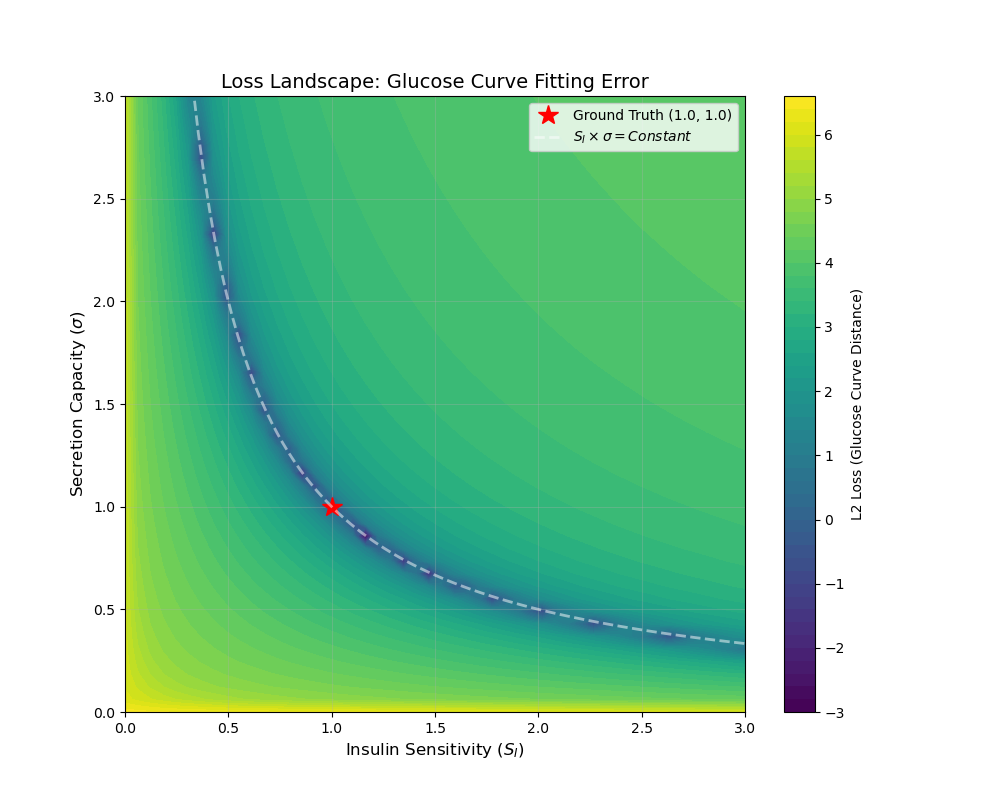
\includegraphics[width=0.78\linewidth]{figures/ogtt_loss_landscape.png}
    \caption{OGTT glucose-only loss landscape in the $(S_I,\sigma)$ plane.
    A pronounced valley indicates that multiple parameter pairs yield nearly indistinguishable glucose trajectories.
    In particular, near-optimal solutions concentrate along curves of approximately constant product $S_I\sigma\approx c$,
    suggesting weak identifiability under glucose-only observations.}
    \label{fig:ogtt-loss-landscape}
\end{figure}

A representative phenomenon is that near-optimal solutions concentrate along curves of the form $S_I\sigma \approx c$ for some constant $c$
depending on the trajectory.
In such a regime, a dataset may contain multiple distinct parameter labels that are consistent with essentially the same observed glucose features.
As a result, even in the population limit, mapping glucose-only features to a unique parameter pair can be ill-posed.

\subsection{Regression-to-mean under MSE and model collapse}
\label{subsec:correctness-mean}

We formalize the above intuition using a standard property of squared-loss regression.

\begin{proposition}[Squared-loss regression yields a conditional mean]\cite{bishop2006prml,hastie2009esl}
\label{prop:cond-mean}
Let $(\mathbf{u},\theta)$ be random variables with $\mathbb{E}\|\theta\|_2^2<\infty$.
Among all measurable functions $g(\mathbf{u})$ minimizing the risk
$
\mathbb{E}\big[\|\theta-g(\mathbf{u})\|_2^2\big],
$
an optimal solution is given by $g^\star(\mathbf{u})=\mathbb{E}[\theta\mid \mathbf{u}]$ (a.s.).
\end{proposition}

\begin{proof}
Fix $\mathbf{u}$ and minimize $\mathbb{E}[\|\theta-g\|_2^2\mid \mathbf{u}]$ over $g\in\mathbb{R}^p$.
Expanding the square shows the unique minimizer is the conditional mean.
\end{proof}

In the OGTT setting, $\mathbf{u}$ is constructed from glucose-only observations (and their derivative features).
When $(S_I,\sigma)$ is not uniquely determined by glucose, the conditional distribution $\theta\mid\mathbf{u}$ can be broad and multimodal.
Consequently, the conditional-mean predictor $\mathbb{E}[\theta\mid\mathbf{u}]$ may lie in the interior of the non-identifiability valley
(e.g., near a ``mean'' point on the curve $S_I\sigma\approx c$) rather than recovering the ground-truth pair.

This provides a principled explanation for the model-collapse behavior observed in our experiments:
the learned predictions concentrate on a low-dimensional set that does not match the true joint distribution of $(S_I,\sigma)$,
even when marginal or projected metrics appear accurate.

This observation also highlights a potential pitfall in evaluation:
metrics computed on individual parameter coordinates (or other low-dimensional projections) can appear favorable even when the predicted \emph{joint}
distribution over $(S_I,\sigma)$ is severely distorted.
For this reason, in Section~\ref{sec:experiments} we complement coordinate-wise errors with (i) joint-distribution diagnostics (e.g., scatter plots of
predicted vs.\ true pairs) and (ii) loss-landscape visualizations such as Figure~\ref{fig:ogtt-loss-landscape}.

\subsection{Takeaway}
\label{subsec:correctness-takeaway}

In summary, contractive fixed-point inference guarantees stable and efficient convergence (Section~\ref{sec:convergence}),
but correctness depends on whether the supervised learning signal can make $T(\theta_{\mathrm{true}};\mathbf{u})\approx \theta_{\mathrm{true}}$.
For OGTT with glucose-only observations, structural or practical non-identifiability leads to label ambiguity, and MSE training selects a conditional-mean
solution that can be far from any individual ground truth.
This limitation is inherent to the observation scheme and motivates additional information or priors, which we discuss in Section~\ref{sec:discussion}.

% Section 8 (Feasibility: identifiability / observability -- organizing principle for the experiments):
\section{Feasibility: Identifiability and Observability Analysis}
\label{sec:identifiability}

Algorithmic convergence of the fixed-point iteration guarantees mathematical stability, but it does not ensure correct parameter recovery if the underlying inverse problem is structurally ill-posed. In this section, we analyze the structural identifiability of our benchmark systems using the nonlinear observability framework of Hermann and Krener \cite{hermann1977nonlinear}.

\subsection{Nonlinear Observability Framework}
We formulate parameter identifiability as a state observability problem by augmenting the state space. Let $\mathbf{x} \in \mathbb{R}^d$ be the system state and $\theta \in \mathbb{R}^p$ be the constant unknown parameters. We define the augmented state $\mathbf{z} = [\mathbf{x}^\top, \theta^\top]^\top \in \mathcal{M} \subseteq \mathbb{R}^{m}$, where $m = d+p$. The augmented dynamics and observation map are:
\begin{equation}
    \dot{\mathbf{z}} = F(\mathbf{z}) = \begin{bmatrix} f(\mathbf{x}, \theta) \\ \mathbf{0} \end{bmatrix}, \quad \mathbf{x}_{obs} = \tilde{h}(\mathbf{z}) = h(\mathbf{x}).
\end{equation}
Following Hermann and Krener, we construct the observability map $\Phi(\mathbf{z}): \mathcal{M} \to \mathbb{R}^{m \times d_{obs}}$ using successive Lie derivatives of the observation function $\tilde{h}$ along the vector field $F$:
\begin{equation}
    \Phi(\mathbf{z}) = \begin{bmatrix} \tilde{h}(\mathbf{z}) \\ L_{F} \tilde{h}(\mathbf{z}) \\ \vdots \\ L_{F}^{m-1} \tilde{h}(\mathbf{z}) \end{bmatrix},
\end{equation}
where $L_F \tilde{h}(\mathbf{z}) = \nabla_{\mathbf{z}} \tilde{h}(\mathbf{z}) \cdot F(\mathbf{z})$. 
The local observability matrix is defined as the Jacobian $\mathbf{O}(\mathbf{z}) := \nabla_{\mathbf{z}} \Phi(\mathbf{z})$. If $\mathbf{O}(\mathbf{z})$ has full rank $m$, the system satisfies the observability rank condition, meaning the observation map is locally a diffeomorphism, and the full augmented state $\mathbf{z}$ (including parameters $\theta$) can be uniquely reconstructed from the observations.

\subsection{SIR: Exact Observability via Lie Derivatives}
For the SIR compartmental model of epidemic dynamics~\cite{kermack1927contribution}, the recovered population $R$ is strictly determined by the conservation law ($N = S+I+R$). Thus, the effective augmented state is $\mathbf{z} = [S, I, \beta, \gamma]^\top \in \mathbb{R}^4$. Under the partial observation setting, only the susceptible population is observed, yielding $\tilde{h}(\mathbf{z}) = S$. 

We explicitly construct the $4 \times 4$ observability matrix by computing the sequence of Lie derivatives along the augmented vector field $F(\mathbf{z}) = [-\beta \frac{SI}{N}, \beta \frac{SI}{N} - \gamma I, 0, 0]^\top$. The first two gradient vectors are derived as:
\begin{align}
    \nabla_{\mathbf{z}} L_{F}^0 \tilde{h}(\mathbf{z}) &= [1, 0, 0, 0], \\
    \nabla_{\mathbf{z}} L_{F}^1 \tilde{h}(\mathbf{z}) &= \left[-\frac{\beta I}{N}, -\frac{\beta S}{N}, -\frac{SI}{N}, 0\right].
\end{align}
Continuing this process up to $L_F^3 \tilde{h}(\mathbf{z})$ systematically embeds the nonlinear interactions of $S, I, \beta$, and $\gamma$ into the rows of $\mathbf{O}(\mathbf{z})$. Evaluating the determinant of the resulting matrix confirms that $\text{rank } \mathbf{O}(\mathbf{z}) = 4$ for generic states $\mathbf{z}$. This direct algebraic calculation rigorously proves that the SIR system is structurally identifiable from $S(t)$ alone. The complete step-by-step derivation of the observability matrix is provided in Appendix \ref{app:obs-sir}.

\subsection{Lotka-Volterra: Unidentifiability via Symbolic Arithmetic}
For the Lotka--Volterra predator--prey system~\cite{lotka1925elements,volterra1927fluctuations}, the augmented state expands to dimension $m = 6$, given by $\mathbf{z} = [x, y, \alpha, \beta, \delta, \gamma]^\top$. The observation function isolates the prey population, $\tilde{h}(\mathbf{z}) = x$.

Constructing the corresponding $6 \times 6$ observability matrix $\mathbf{O}(\mathbf{z})$ requires evaluating up to the 5th-order Lie derivative ($L_F^5 \tilde{h}$). Due to the exponential growth of polynomial cross-terms, manual derivation becomes intractable. Therefore, we utilize symbolic algebraic computation (via SymPy) to generate the gradients and assemble $\mathbf{O}(\mathbf{z})$. The symbolic evaluation analytically confirms that:
\begin{equation}
    \text{rank } \mathbf{O}(\mathbf{z}) = 5 < 6.
\end{equation}
Because the algebraic rank is strictly less than the dimension of the augmented state space, the system is not locally observable from prey-only observations. As illustrated in Figure \ref{fig:lv_unidentifiable}, this rank deficiency implies the existence of distinct combinations of hidden predator trajectories and interaction parameters that map to the exact same prey trajectory $\mathbf{x}_{obs}(t)$. The SymPy code utilized for this exact algebraic derivation is included in Appendix \ref{app:obs-lv}.

\begin{figure}[htbp]
  \centering
  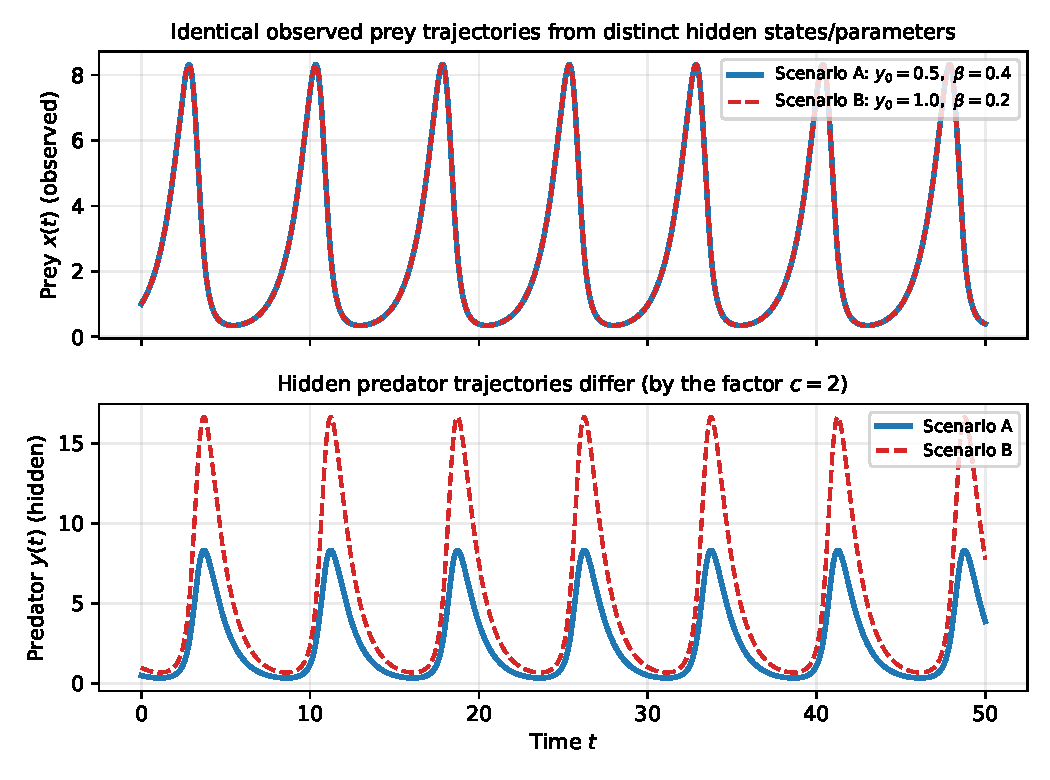
\includegraphics[width=0.82\textwidth]{figures/lv_nonident.pdf}
  %\framebox{\parbox{0.8\textwidth}{\centering
  %  \vspace{3cm}
  %  \textbf{} \\
  %  \small\textit{Identical prey observations $x(t)$ (top) from completely different hidden predator states $y(t)$ and parameter $\beta$ (bottom).}
  %  \vspace{3cm}
  %}}
  \caption{Structural unidentifiability in the Lotka-Volterra model. Scenario A ($x_0=1.0, y_0=0.5, \beta=0.4$) and Scenario B ($x_0=1.0, y_0=1.0, \beta=0.2$) produce identical observable trajectories for the prey $\mathbf{x}_{obs}(t)$ (top), despite originating from completely different hidden predator states and parameters (bottom). This algebraic indistinguishability proves that the full system cannot be identified from partial observations alone.}
  \label{fig:lv_unidentifiable}
\end{figure}

\subsection{OGTT: Jacobian Approximation and Theoretical Observability}
\label{subsec:ident-ogtt}
For the OGTT (oral glucose tolerance test) glucose--insulin minimal model~\cite{ha2025disposition}, the augmented state is
\begin{equation*}
\mathbf{z} = [G, I, N_5, N_6, S_I, \sigma]^\top \in \mathbb{R}^6, \qquad \mathbf{x}_{obs} = \tilde{h}(\mathbf{z}) = G .
\end{equation*}
Due to the high dimensionality and nested recurrences in the vector field, deriving $\mathbf{O}(\mathbf{z})$ even via symbolic computation is intractable.

Instead, we employ a Jacobian-based numerical approximation. The Taylor expansion of the observation $\mathbf{x}_{obs}(t)$ near $t=0$ can be expressed using Lie derivatives:
\begin{equation}
    \mathbf{x}_{obs}(t) = L_{F}^0 \tilde{h}(\mathbf{z}(0)) + t L_{F}^1 \tilde{h}(\mathbf{z}(0)) + \frac{t^2}{2!} L_{F}^2 \tilde{h}(\mathbf{z}(0)) + \dots
\end{equation}
Taking the gradient with respect to the initial augmented state $\mathbf{z}(0)$ and truncating at dimension $d=6$, the Jacobian $\mathbf{J} = \nabla_{\mathbf{z}(0)} \mathbf{x}_{obs}(\mathbf{t})$ evaluated at $T \ge 6$ discrete time points factors into:
\begin{equation}
    \mathbf{J} \approx \underbrace{\begin{bmatrix} 1 & t_1 & \dots & \frac{t_1^{d-1}}{(d-1)!} \\ \vdots & \vdots & \ddots & \vdots \\ 1 & t_T & \dots & \frac{t_T^{d-1}}{(d-1)!} \end{bmatrix}}_{\mathbf{T}} \underbrace{\begin{bmatrix} \nabla_{\mathbf{z}} L_{F}^0 \tilde{h}(\mathbf{z}(0)) \\ \vdots \\ \nabla_{\mathbf{z}} L_{F}^{d-1} \tilde{h}(\mathbf{z}(0)) \end{bmatrix}}_{\mathbf{O}(\mathbf{z}(0))}.
\end{equation}
Since the Vandermonde matrix $\mathbf{T}$ has full column rank for distinct time points, $\text{rank}(\mathbf{J}) = \text{rank}(\mathbf{O}(\mathbf{z}))$. We estimate $\text{rank}(\mathbf{J})$ using finite differences and Singular Value Decomposition (SVD), carefully normalizing the scale of each variable. 

The SVD yields six strictly positive singular values ($\varsigma_1 \approx 1.2\times 10^{2} \dots \varsigma_6 \approx 1.5\times 10^{-3}$; Figure~\ref{fig:ogtt_sensitivity}, left), all well above machine zero (we write $\varsigma$ for singular values to avoid collision with the parameter $\sigma$). This confirms that $\text{rank}(\mathbf{O}) = 6$. Theoretically, under idealized conditions with sufficient time steps and high-order derivative information, the OGTT system is structurally identifiable from glucose alone.

\subsection{Bridging Theory and Practice: The Ill-Conditioning of OGTT}
While theoretically identifiable, the SVD spectrum reveals a critical practical challenge. The singular values span roughly five orders of magnitude, indicating that the Jacobian $\mathbf{J}$ is severely ill-conditioned.

\begin{figure}[htbp]
  \centering
  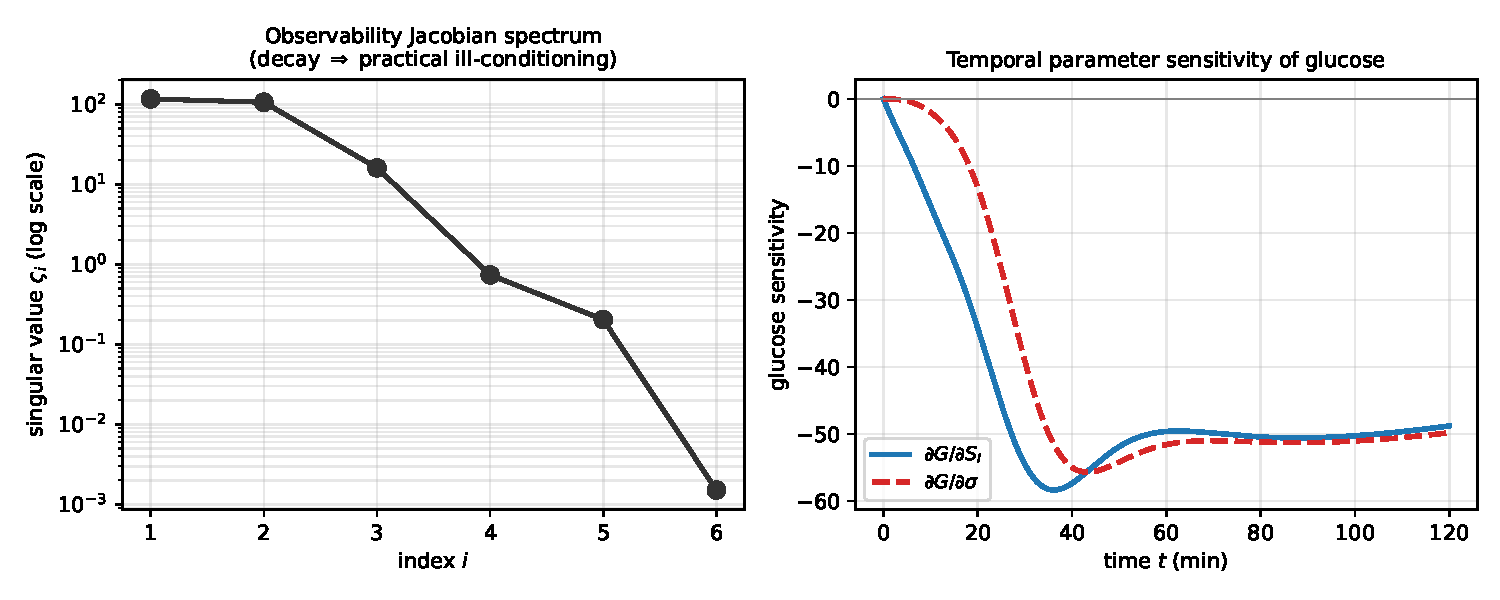
\includegraphics[width=0.92\textwidth]{figures/ogtt_illcond.pdf}
  %\framebox{\parbox{0.8\textwidth}{\centering
  %  \vspace{3cm}
  %  \textbf{} \\
  %  \small\textit{(Left) Singular value spectrum showing steep decay. (Right) Normalized sensitivity dynamics of $S_I$ and $\sigma$ over time.}
  %  \vspace{3cm}
  %}}
  \caption{Ill-conditioning and parameter sensitivity in the OGTT model. (Left) The singular values of the Jacobian decay rapidly, indicating practical unidentifiability despite theoretical full rank. (Right) The temporal sensitivity of glucose to $S_I$ and $\sigma$. Early dynamics ($<30$ min) are dominated by $S_I$, while later dynamics entangle the effects of both parameters.}
  \label{fig:ogtt_sensitivity}
\end{figure}

This ill-conditioning manifests temporally. As shown in Figure \ref{fig:ogtt_sensitivity} (Right), the sensitivity of glucose to insulin sensitivity ($\partial G / \partial S_I$) rises first, becoming strongest within the first $30$--$40$ minutes. The influence of $\beta$-cell function ($\partial G / \partial \sigma$) instead builds up more slowly, along a sigmoid-like profile. In the later stages, the two sensitivities become comparable and the coupled influence of both parameters dictates the glucose trajectory. Under a uniform 30-minute sampling grid without continuous flow information, the neural network struggles to disentangle these intertwined sensitivities. This translates the theoretically full-rank system into a practically unidentifiable regime, severely limiting the precise joint recovery of $(S_I, \sigma)$ and paving the way for the regression-to-mean phenomenon.


% Section 9 (Experiments):
\section{Experiments}
\label{sec:experiments}

We evaluate the iterative fixed-point estimator on three dynamical systems that span the
identifiability spectrum predicted a priori by the observability analysis of
Section~\ref{sec:identifiability}: the epidemiological SIR model (structurally observable), the
ecological Lotka--Volterra model (observability matrix rank-deficient in one parameter direction),
and the physiological OGTT glucose--insulin model (weakly identifiable, with only the product
$mDI=S_I\sigma$ recoverable from glucose~\cite{ha2025disposition}). For each system we train the two networks $H_\phi,P_\psi$
by teacher forcing and compare the converged fixed point $\theta^*(\mathbf{x}_\mathrm{obs})$ against a
\emph{direct-regression baseline} --- a single network $x_\mathrm{obs}\mapsto\theta$ of matched
capacity trained by MSE on the identical data split. The comparison is diagnostic rather than
competitive: because both estimators minimize a squared loss, both are driven toward the conditional
mean (Proposition~\ref{prop:optimal_predictor}), so the baseline isolates the \emph{structural}
component of the error (Remark~\ref{rem:decomposition}(i)) from the iterative operator's own
approximation gap (ii).

\paragraph{Protocol.} Synthetic trajectories are generated by numerical integration under sparse,
partial observation (SIR/LV: $2\times10^4$ samples; OGTT: $5\times10^4$). Spectral normalization is
applied with a per-layer margin yielding a verified contraction constant
$\mathrm{Lip}_\mathcal{T}\approx 0.6<1$ (Section~\ref{subsec:sn}); inference uses $K=10$ fixed-point
iterations. We report coordinate-wise RMSE (physical units) and Pearson correlation $r$ between true
and predicted parameters; because RMSE is scale-dependent across systems, $r$ is the primary
scale-invariant indicator of whether a parameter is recovered at all.

\begin{table}[t]
\centering
\caption{Parameter recovery (RMSE\,/\,Pearson $r$) on synthetic test data. The direct baseline
recovers structurally identifiable parameters nearly perfectly ($r\!\approx\!0.98$); it fails
exactly on the observability-predicted non-identifiable directions (LV $\beta$; OGTT
$S_I,\sigma$ individually). The iterative estimator converges but exhibits an additional
approximation gap even where the problem is identifiable (SIR).}
\label{tab:recovery}
\begin{tabular}{llcc}
\hline
System & Parameter & Iterative (RMSE\,/\,$r$) & Direct baseline (RMSE\,/\,$r$) \\
\hline
SIR       & $\beta$   & $0.108\,/\,0.66$ & $\mathbf{0.026\,/\,0.98}$ \\
(wide)    & $\gamma$  & $0.105\,/\,0.68$ & $\mathbf{0.055\,/\,0.92}$ \\
\hline
Lotka--   & $\alpha$  & $0.102\,/\,0.54$ & $\mathbf{0.014\,/\,0.99}$ \\
Volterra  & $\beta$   & $0.115\,/\,0.02$ & $0.113\,/\,0.22$ \\
          & $\delta$  & $0.089\,/\,0.84$ & $\mathbf{0.012\,/\,0.99}$ \\
          & $\gamma$  & $0.096\,/\,0.62$ & $\mathbf{0.020\,/\,0.99}$ \\
\hline
OGTT      & $S_I$     & $0.265\,/\,0.65$ & $0.212\,/\,0.76$ \\
          & $\sigma$  & $0.338\,/\,0.65$ & $0.254\,/\,0.82$ \\
\hline
\end{tabular}
\end{table}

Table~\ref{tab:recovery} summarizes all runs; the following subsections read it through the theory.

\subsection{SIR: an identifiability control that isolates the operator gap}
\label{subsec:exp-sir}

The augmented SIR system satisfies the observability rank condition from its sparse partial
observations of $S(t)$ (Section~\ref{sec:identifiability}), so the conditional variance
$\operatorname{Var}(\theta\mid\mathbf{x}_\mathrm{obs})$ is negligible and the structural term
(Remark~\ref{rem:decomposition}(i)) vanishes. Consistently, the direct baseline recovers $(\beta,\gamma)$
almost exactly ($r=0.98,0.92$). The iterative estimator, although it converges to a unique fixed point
(Theorem~\ref{thm:contraction}), attains only $r=0.66,0.68$ (Figure~\ref{fig:sir-scatter}): predictions
concentrate in a narrow band and $\mathcal{R}_0$ saturates. Since the problem is identifiable, this
residual bias cannot be structural; it is precisely the operator-approximation term
(Remark~\ref{rem:decomposition}(ii)) --- the composition $P_\psi\!\circ\!H_\phi$ does not preserve
$\theta$ perfectly, keeping the one-step residual $\varepsilon(\mathbf{x}_\mathrm{obs})$ bounded away from
zero. SIR thus serves as a control that exhibits (ii) in isolation, and cautions against reading the
iterative estimator's accuracy as evidence about identifiability. This gap is exactly the cost of the
reconstruction detour identified in Proposition~\ref{prop:ceiling}: the direct regressor, which maps
$\mathbf{x}_\mathrm{obs}$ to $\theta$ without reconstructing the hidden state, reaches the
conditional-mean ceiling far more closely ($r\approx0.98$) than the iteration ($r\approx0.66$), on the
identical data. (The same picture holds on a narrow-range variant matching commonly reported values,
where the baseline reaches $r\approx0.99$ and the iteration $r\approx0.4$--$0.5$.)

To confirm that the gap is driven by the difficulty of reconstructing the hidden state --- and not by
non-identifiability --- we sweep the observation density (Figure~\ref{fig:sir-density}). As the number
of observation points increases from $4$ to $30$, the iterative estimator's recovery improves
monotonically ($r_\beta: 0.66\!\to\!0.71\!\to\!0.75\!\to\!0.78$): denser observations make the hidden
trajectory easier to reconstruct, shrinking $\varepsilon$ and, by Lemma~\ref{lem:error_bound}, the
fixed-point error. This validates the correctness bound as non-vacuous. Yet the improvement plateaus
well below the direct-regressor ceiling ($r\approx0.98$, already at $4$ points), consistent with
Proposition~\ref{prop:ceiling}: the reconstruction detour retains a residual cost that observation
density alone does not remove. Correctness is approached, but not achieved, precisely in the regime
--- dense, well-conditioned observation --- that the sparse-and-partial premise of this paper excludes.

\begin{figure}[t]
\centering
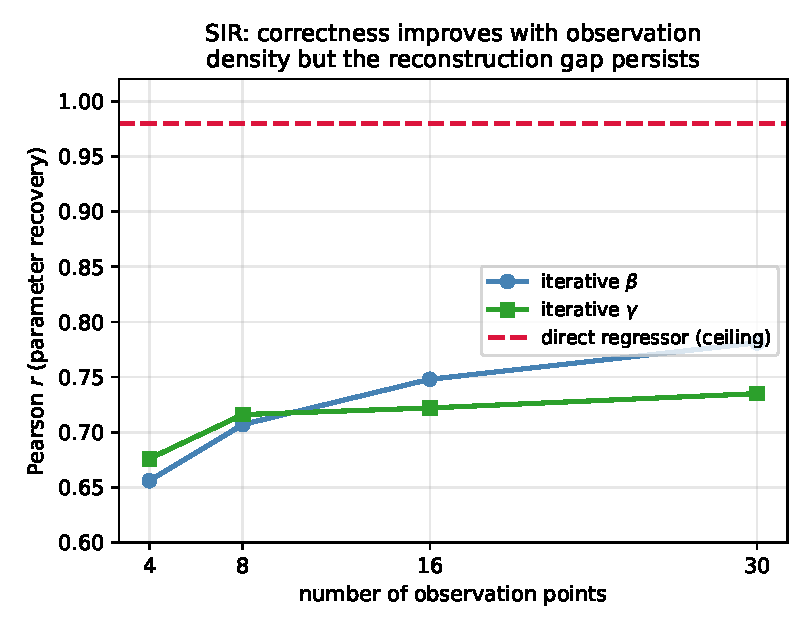
\includegraphics[width=0.6\linewidth]{figures/exp/sir_density_sweep.pdf}
\caption{SIR observation-density sweep (identifiable regime, unknown-hidden-state setting). The
iterative estimator's parameter recovery improves monotonically with the number of observation points
--- validating that the fixed-point error is governed by the one-step residual
(Lemma~\ref{lem:error_bound}) --- but plateaus below the direct-regressor ceiling
(Proposition~\ref{prop:ceiling}): denser data eases hidden-state reconstruction yet does not remove the
detour cost.}
\label{fig:sir-density}
\end{figure}

\begin{figure}[t]
\centering
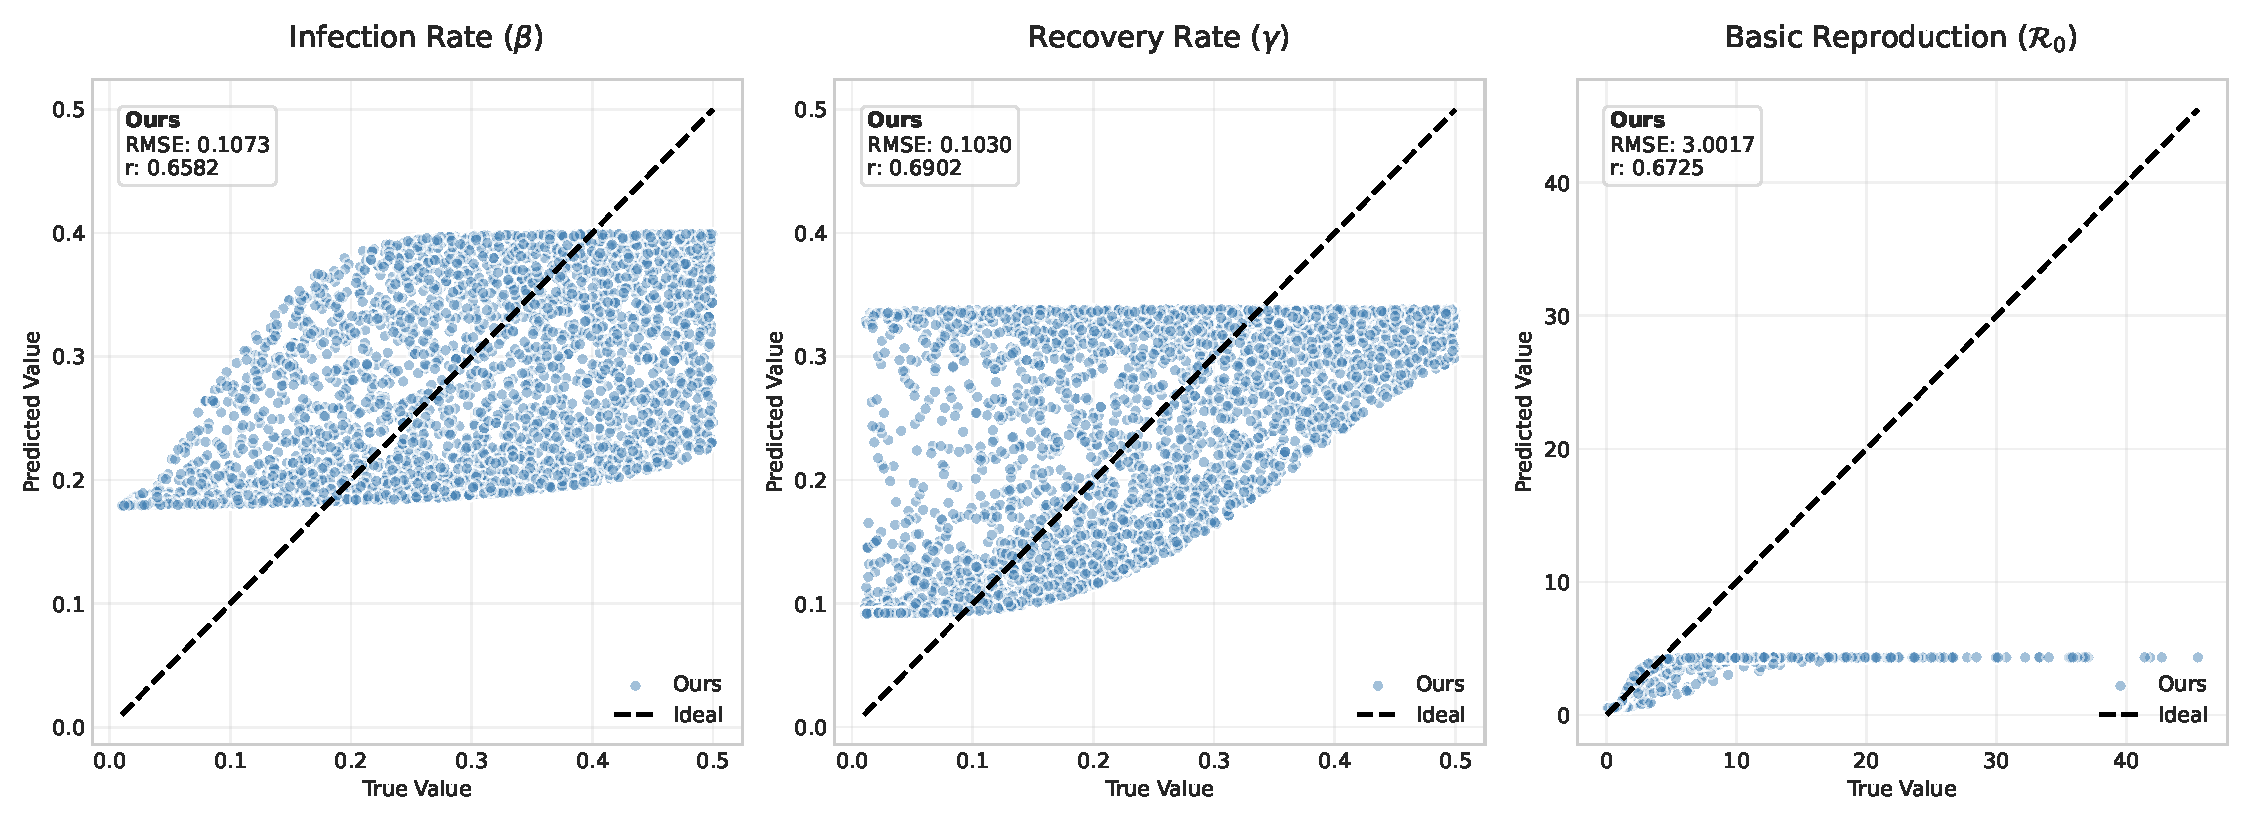
\includegraphics[width=0.92\linewidth]{figures/exp/sir_scatter_wide_iter.pdf}
\caption{SIR parameter recovery, iterative estimator. Predictions (blue) versus ground truth for
$\beta,\gamma,\mathcal{R}_0$. Despite guaranteed convergence, predictions compress toward a central
band and $\mathcal{R}_0$ saturates --- the operator-approximation gap of
Remark~\ref{rem:decomposition}(ii), present even though SIR is identifiable (cf. the direct baseline,
$r\approx0.98$).}
\label{fig:sir-scatter}
\end{figure}

\subsection{Lotka--Volterra: observability predicts which parameters are recoverable}
\label{subsec:exp-lv}

For prey-only observation the augmented Lotka--Volterra observability matrix is rank-deficient
($\operatorname{rank}\mathbf{O}=5<6$; Section~\ref{sec:identifiability}), and the deficient direction
corresponds to the interaction parameter $\beta$. The experiment confirms this prediction sharply: the
direct baseline recovers $\alpha,\delta,\gamma$ nearly perfectly ($r=0.99,0.99,0.99$) but collapses on
$\beta$ ($r=0.22$), while every other coordinate remains recoverable (Figure~\ref{fig:lv-scatter}).
Thus the a-priori observability rank predicts, parameter by parameter, exactly where estimation is
possible --- turning ``the method sometimes fails'' into a quantitative statement about the problem.
The iterative estimator recovers the same identifiable coordinates with the additional bias of
(ii) ($r=0.54$--$0.84$) and, like the baseline, cannot recover the unobservable $\beta$.

\begin{figure}[t]
\centering
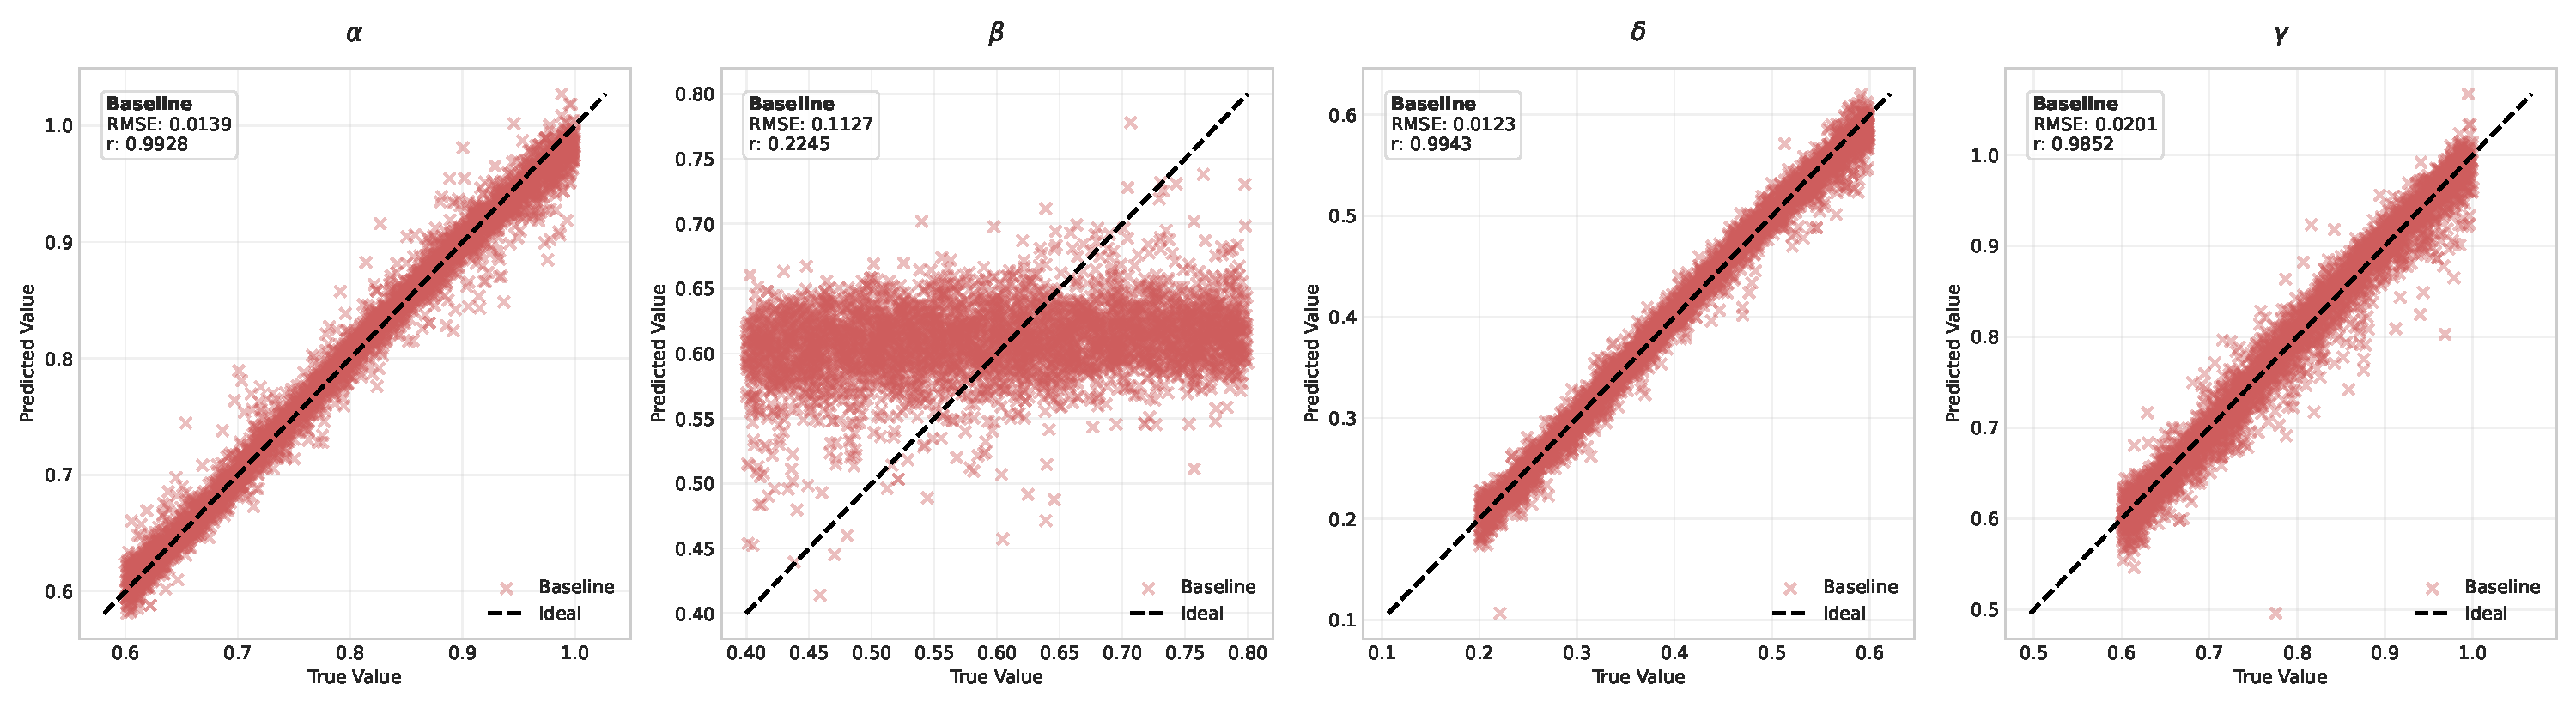
\includegraphics[width=0.92\linewidth]{figures/exp/lv_scatter_base.pdf}
\caption{Lotka--Volterra recovery, direct baseline. Three parameters are recovered nearly perfectly
($\alpha,\delta,\gamma$: $r\approx0.99$); the interaction parameter $\beta$ is not
($r=0.22$)---exactly the direction the observability matrix flags as rank-deficient
(Section~\ref{sec:identifiability}).}
\label{fig:lv-scatter}
\end{figure}

\subsection{OGTT: structural collapse onto an off-fiber locus}
\label{subsec:exp-ogtt}

Under glucose-only observation, $\theta=(S_I,\sigma)$ is identifiable only through the product
$mDI=S_I\sigma$ (Section~\ref{sec:identifiability}); the conditional distribution along each fiber
$\{S_I\sigma=c\}$ is non-degenerate, so the structural term (i) dominates. This is the regime targeted
by Corollary~\ref{cor:lower_bound} and Proposition~\ref{prop:off_fiber}.

Figure~\ref{fig:ogtt-collapse} makes the predicted behavior visible. \emph{(Left)} the joint
distribution of predictions collapses from the two-dimensional ground-truth cloud onto an essentially
one-dimensional locus --- the joint-distribution collapse of Corollary~\ref{cor:lower_bound}.
\emph{(Center)} the identifiable product $\log(S_I\sigma)$ (the ``stiff'' direction) is recovered, its
density matching the ground truth (Pearson $r=0.93$ for the iterative estimator, $r=0.99$ for the
baseline). \emph{(Right)} the two individual coordinates are \emph{both} unrecovered, and to the same
degree: $r(S_I)=r(\sigma)=0.65$ for the iterative estimator and $r(S_I)=0.76,\ r(\sigma)=0.82$ for the
baseline. Neither coordinate is privileged --- only the product is pinned down, while the estimate is
free to slide along the fiber. The signature predicted by Corollary~\ref{cor:off_fiber_product} ---
that the recovered product is biased relative to the true identifiable statistic and the estimate
leaves the physical fiber --- is directly observed. Crucially, the direct baseline exhibits the
\emph{same} structural collapse (it too recovers the product but not the individual coordinates),
confirming that the limitation binds any squared-loss point estimator and is not an artifact of the
fixed-point iteration.

\begin{figure}[t]
\centering
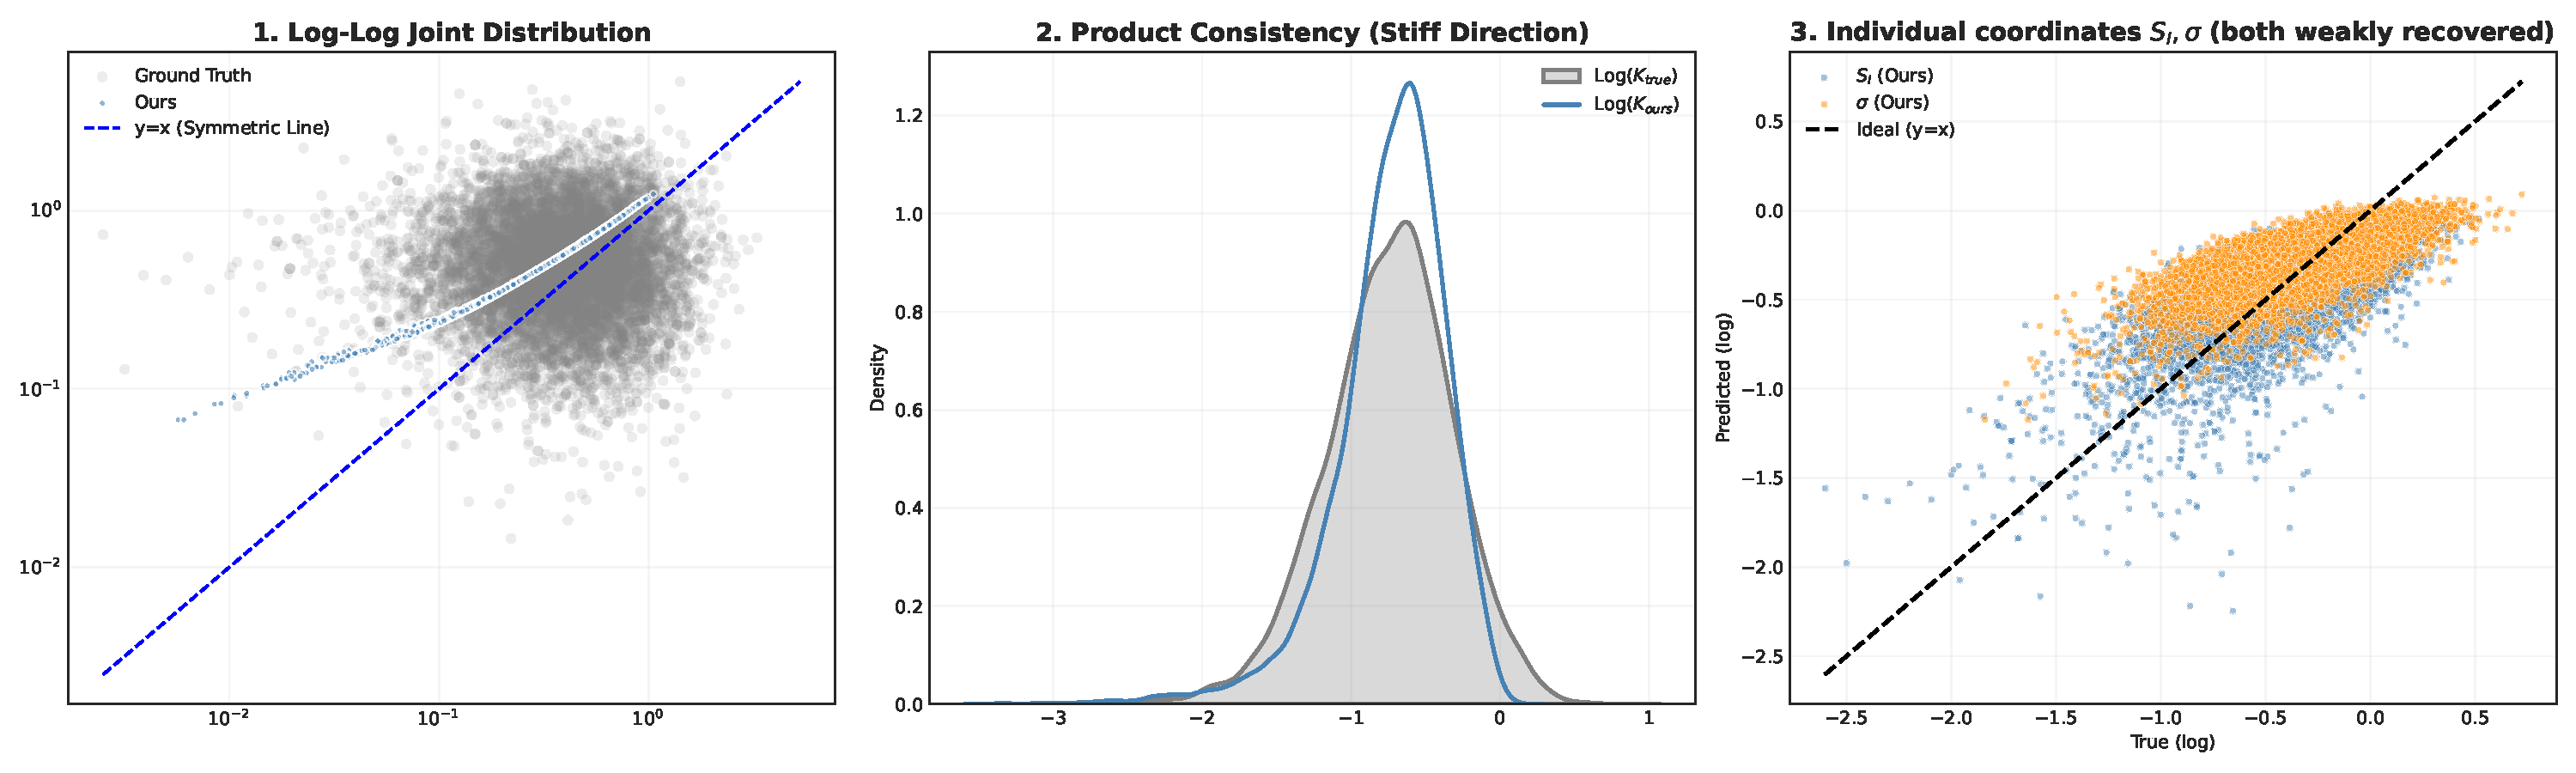
\includegraphics[width=\linewidth]{figures/exp/ogtt_collapse_iter.pdf}
\caption{OGTT joint-distribution collapse (iterative estimator; the direct baseline is
qualitatively identical). \emph{Left:} predictions (blue) collapse the 2-D ground-truth cloud (grey)
onto a 1-D locus. \emph{Center:} the identifiable product $S_I\sigma$ (stiff direction) is recovered
($r=0.93$). \emph{Right:} the two individual coordinates $S_I$ and $\sigma$ are both unrecovered and to
the same degree ($r=0.65$ each), neither privileged --- the estimate slides freely along the fiber.
This realizes the regression-to-mean of Corollary~\ref{cor:lower_bound} and the off-fiber conditional
mean of Proposition~\ref{prop:off_fiber} / Corollary~\ref{cor:off_fiber_product}.}
\label{fig:ogtt-collapse}
\end{figure}

\subsection{Convergence and the role of the contraction margin}
\label{subsec:exp-convergence}

Figure~\ref{fig:ogtt-phase} visualizes the fixed-point dynamics in the $(S_I,\sigma)$ plane:
trajectories launched from widely separated initializations all converge to a \emph{single} fixed
point (Theorem~\ref{thm:contraction}), yet that fixed point does not coincide with the ground truth ---
a direct picture of ``convergence $\neq$ correctness.'' The annotated one-step residual
$\varepsilon=0.08$ and fixed-point error $\|\theta^*-\theta^{\mathrm{true}}\|=0.11$ are consistent with
the bound $\varepsilon/(1-\mathrm{Lip}_\mathcal{T})$ of Lemma~\ref{lem:error_bound}.

Finally, we vary the spectral-normalization margin. Across per-layer targets giving verified
contraction constants $\mathrm{Lip}_\mathcal{T}\in\{0.28,0.60,0.89,0.92\}$, parameter accuracy is
essentially flat (SIR $\beta$: RMSE $0.11$--$0.11$, $r\approx0.64$--$0.68$); without spectral
normalization the composite Lipschitz constant is $\gg 1$, the iteration fails to contract, and
accuracy collapses ($r<0$). This matches the theory: spectral normalization supplies the convergence
\emph{guarantee}, but within the contractive regime the residual error is set by
$\varepsilon(\mathbf{x}_\mathrm{obs})$ --- the structural and operator terms of
Remark~\ref{rem:decomposition} --- not by the size of the margin.

\begin{figure}[t]
\centering
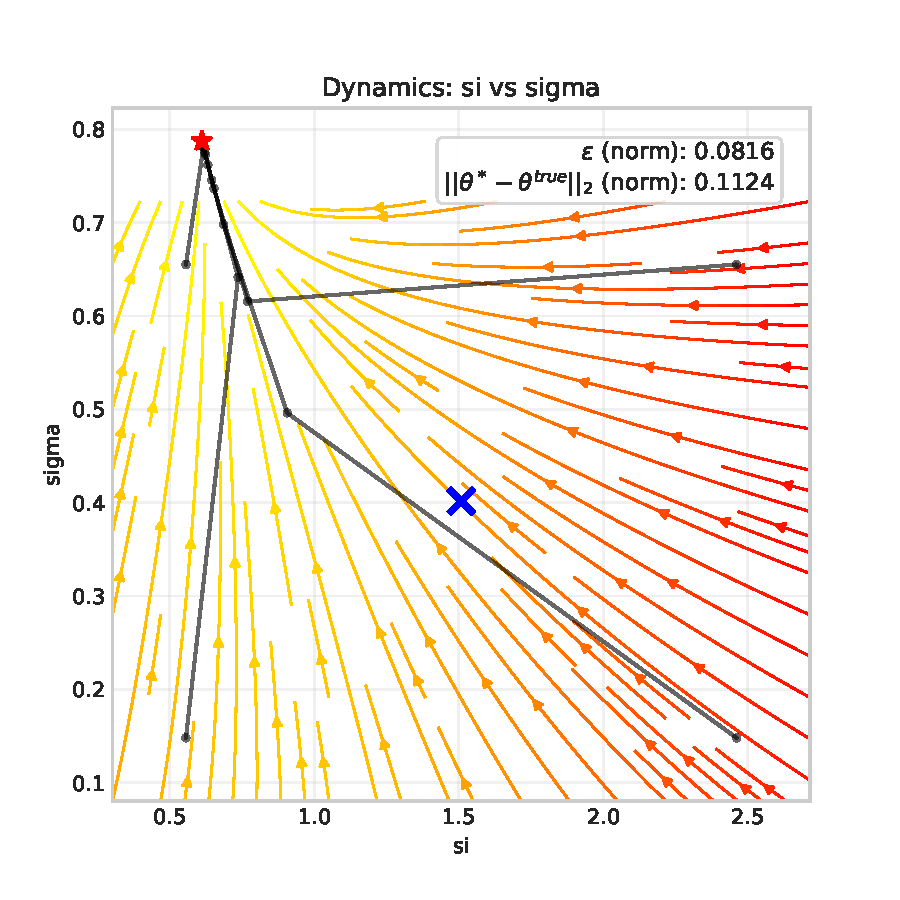
\includegraphics[width=0.62\linewidth]{figures/exp/ogtt_phase.pdf}
\caption{Fixed-point dynamics for OGTT in the $(S_I,\sigma)$ plane. Trajectories from four
initializations converge to one fixed point (red star), which differs from the ground truth (blue
cross): convergence does not imply correctness. Annotations report the one-step residual $\varepsilon$
and the fixed-point error, consistent with Lemma~\ref{lem:error_bound}.}
\label{fig:ogtt-phase}
\end{figure}

\paragraph{A note on distribution shift.} On real clinical OGTT measurements (out of the synthetic
training distribution), the direct baseline's predictions diverge under denormalization, whereas the
iterative estimator's strongly biased output remains bounded. We record this as an observation about
the two estimators' behavior under distribution shift; a robustness claim is beyond the scope of the
present, characterization-focused study.

% Section 10 (Discussion: positioning vs other point estimators; motivation for distributional inference):
\section{Discussion}
\label{sec:discussion}

It is important to locate our negative result correctly: the limitation we establish is a property of the \emph{problem}, not of the decoupled fixed-point construction in particular. Because the conditional-mean ceiling of Proposition~\ref{prop:ceiling} applies to \emph{any} estimator that is a function of $\mathbf{x}_\mathrm{obs}$ and is trained under squared loss, it binds the direct regressor and any amortized point estimator exactly as it binds our iteration. Methods built on other principles fail as well, but in different ways. Likelihood-based estimators --- nonlinear least squares, or an EM scheme that alternates between inferring the latent trajectory and updating the parameter --- target a maximizer of the observation likelihood rather than a conditional mean; under non-identifiability the likelihood is flat along the fiber $\mathcal{F}_c$, so such methods converge to \emph{some} admissible fiber point, but a non-unique, initialization-dependent one, with no indication of the residual ambiguity. Thus squared-loss methods regress off the fiber to a biased mean, while likelihood-based methods land on the fiber but cannot single out the true solution; neither returns a correct, unique estimate, because the information required to do so is simply absent from $\mathbf{x}_\mathrm{obs}$.

This dichotomy points to what a satisfactory answer must look like. When a problem is non-identifiable, the object genuinely determined by the observation is not a single parameter but a set --- the fiber, together with the distribution induced on it by the prior and the observation noise. Any method that insists on returning one point must therefore either bias the estimate (squared loss) or make an arbitrary choice (likelihood), and no amount of algorithmic refinement removes this. The natural remedy is to lift inference from point estimates to \emph{distributions}: to characterize the posterior $p(\theta \mid \mathbf{x}_\mathrm{obs})$, which correctly represents the identifiable statistic ($mDI = S_I\sigma$ for OGTT), the residual uncertainty along the fiber, and the physical admissibility that point estimators forfeit. Developing such a distribution-valued amortized inference procedure --- one that retains the decoupled hidden-state structure but replaces the deterministic maps with conditional samplers --- is the direction we pursue in subsequent work, and the ceiling identified here is precisely what it is designed to overcome.




%\section{Conclusions}
%\label{sec:conclusions}

\appendix
%\section{An example appendix}
%\section{Implementation details: OGTT normalization}
\label{app:impl}

This appendix documents preprocessing used in the OGTT experiments.
SIR and Lotka--Volterra experiments use raw simulated values without additional normalization.

\subsection{Dataset-level state normalization}
\label{app:state-norm}

To improve numerical stability, we normalize observed and hidden state values by dataset-level scale factors computed from the training set.
Let $\{x_{\mathrm{obs}}^{(m)}(t_i)\}$ and $\{x_{\mathrm{hid}}^{(m)}(t_i)\}$ denote simulated OGTT training samples at sampling times.
We define
\begin{equation}
\label{eq:app-state-scales}
s_{\mathrm{obs}} := 1.2\cdot \mathrm{Quantile}_{0.999}\!\left(\,|x_{\mathrm{obs}}|\,\right),\qquad
s_{\mathrm{hid}} := 1.2\cdot \mathrm{Quantile}_{0.999}\!\left(\,|x_{\mathrm{hid}}|\,\right),
\end{equation}
where each quantile is taken over all training trajectories and sampling times (and absolute value is applied elementwise).

We normalize the inputs to the neural networks by
\begin{equation}
\label{eq:app-state-norm}
x_{\mathrm{obs}}^{\mathrm{norm}}(t_i)=\frac{x_{\mathrm{obs}}(t_i)}{s_{\mathrm{obs}}},\qquad
x_{\mathrm{hid}}^{\mathrm{norm}}(t_i)=\frac{x_{\mathrm{hid}}(t_i)}{s_{\mathrm{hid}}}.
\end{equation}
When derivative features are used, we apply the same scaling to preserve derivative information up to a global factor:
\begin{equation}
\label{eq:app-deriv-norm}
\widehat{\dot{x}}_{\mathrm{obs}}^{\mathrm{norm}}(t_i)=\frac{\widehat{\dot{x}}_{\mathrm{obs}}(t_i)}{s_{\mathrm{obs}}}.
\end{equation}

\subsection{Parameter normalization and log-transform}
\label{app:param-norm}

For OGTT parameters we use a log transform prior to min--max scaling.
Given a physical parameter vector $\theta\in\mathbb{R}_+^p$, define $\varphi(\theta)=\log(\theta+\varepsilon)$ for a small $\varepsilon>0$.
We use $\varepsilon=10^{-9}$ in the log transform.
Let $\theta_{\min},\theta_{\max}\in\mathbb{R}^p$ be dataset-derived bounds computed from the training set with a $20\%$ margin:
\begin{equation}
\label{eq:app-param-bounds}
\theta_{\min} := \theta_{\min,\mathrm{data}}/1.2,\qquad
\theta_{\max} := 1.2\,\theta_{\max,\mathrm{data}}.
\end{equation}
We map parameters to $[-1,1]^p$ via
\begin{equation}
\label{eq:app-param-norm}
\theta^{\mathrm{norm}}
= 2\,\frac{\varphi(\theta)-\varphi(\theta_{\min})}{\varphi(\theta_{\max})-\varphi(\theta_{\min})}-1.
\end{equation}
At inference, predicted parameters are denormalized back to physical units by inverting \eqref{eq:app-param-norm} and then applying
$\varphi^{-1}(\cdot)=\exp(\cdot)$.

\subsection{Practical notes}
\label{app:practical-notes}

In our implementation, the scale factors $(s_{\mathrm{obs}},s_{\mathrm{hid}})$ and bounds $(\theta_{\min},\theta_{\max})$ are computed once from the training set and
then reused across training and inference to avoid time-dependent rescaling.
%\section{Implementation details: training protocol}
\label{app:impl-train}
\subsection{Hyperparameters and implementation settings}
\label{app:hyperparams}

\begin{table}[t]
\centering
\footnotesize
\setlength{\tabcolsep}{3pt} % 열 간격 줄이기
\renewcommand{\arraystretch}{1.05}
\caption{Hyperparameters used in the experiments. Values are highlighted for easy modification.}
\label{tab:hyperparams}
\begin{tabular}{p{0.18\linewidth} p{0.36\linewidth} p{0.38\linewidth}}
\hline
\textbf{Category} & \textbf{Setting} & \textbf{Value} \\
\hline
System & System / seed / device & \HP{ogtt\_simul}, \HP{42}, \HP{CUDA if available} \\
Data & \#samples / split / batch & \HP{10000}, \HP{0.2}, \HP{512} \\
SDE data & Aug. factor / diffusion scale & \HP{30}, \HP{1.27} \\
Training & Epochs / lr / wd & \HP{10000}, \HP{$10^{-4}$}, \HP{$10^{-4}$} \\
Training & Early stopping (pat., min-$\Delta$) & \HP{200}, \HP{$10^{-6}$} \\
Training & LR schedule & \HP{Plateau: factor 0.9, pat. 20, min lr $10^{-8}$} \\
Training & Grad clip & \HP{$\|g\|\le 1.0$} \\
Features & Derivative / method & \HP{on}, \HP{spline} \\
Loss & Components & \HP{sup. + rec. (w=1,1)} \\
Inference & Iterations & \HP{10} \\
Model & Hidden dims / activation & \HP{[64,64,64]}, \HP{SiLU} \\
Regularize & Spectral norm / power iters & \HP{on}, \HP{5} \\
\hline
\end{tabular}
\end{table}
\noindent\textbf{Note.}
All parameter-learning and convergence analysis are performed in normalized parameter coordinates.
Reported parameter estimates are denormalized to physical units for evaluation.

This appendix summarizes training and inference hyperparameters used in our experiments.

\subsection{Data and batching}
We generate \HPNumSamples\ trajectories for training, with a test split of \HPTestSplit.
Mini-batch training uses batch size \HPBatchSize.

\subsection{Optimization}
We train for up to \HPEpochs\ epochs using AdamW with learning rate \HPLR\ and weight decay \HPWeightDecay.
We apply gradient clipping with maximum norm $1.0$.

Early stopping is enabled (\HPEarlyStop) with patience \HPEarlyPat\ and minimum improvement threshold \HPEarlyDelta.
A ReduceLROnPlateau scheduler is used as described in the codebase.

\subsection{Loss configuration}
Unless otherwise stated, we use the composite objective with components \HPLossCfg.
The recurrent component corresponds to an unrolled training objective (see Section~\ref{sec:loss-design} for discussion, if included).

\subsection{Model architecture and regularization}
Both networks use hidden dimensions \HPHiddenDims\ and activation \HPAct.
Spectral normalization is enabled (\HPSN) and applied to all linear layers.

\subsection{Derivative features and inference iteration}
Derivative features are used (\HPUseDeriv) and computed at inference by the \HPDerivMethod\ method.
The inference iteration uses \HPIter\ fixed steps.
\section{Observability computations for SIR, Lotka--Volterra, and OGTT}
\label{app:observability}

This appendix documents the calculations and code used to support the observability/identifiability statements in
Section~\ref{sec:identifiability}.
We treat parameters as augmented constant states and follow the nonlinear observability framework of Hermann and Krener~\cite{hermann1977nonlinear}.

\subsection{SIR model: Lie-derivative-based observability matrix}
\label{app:obs-sir}

We take the augmented state
\[
z = (S,I,R,\beta,\gamma),
\]
with observation $h(z)=I$.
The vector field for the augmented system is
\[
\Sigma(z) = (\dot{S},\dot{I},\dot{R},0,0)
=
(-\beta S I,\ \beta S I-\gamma I,\ \gamma I,\ 0,\ 0).
\]

We compute Lie derivatives of $h$ along $\Sigma$ and their gradients:
\begin{align*}
L_\Sigma^0 h(z) &= h(z) = I,\\
L_\Sigma^1 h(z) &= \nabla h(z)\cdot \Sigma(z) = \beta S I - \gamma I,\\
L_\Sigma^2 h(z) &= \nabla L_\Sigma^1 h(z)\cdot \Sigma(z),\\
&\vdots
\end{align*}
and assemble the observation map
\[
\Phi(z)
=
\begin{bmatrix}
L_\Sigma^0 h(z)\\
L_\Sigma^1 h(z)\\
\vdots\\
L_\Sigma^{4} h(z)
\end{bmatrix},
\qquad
\mathbf{O}(z) := \nabla_z \Phi(z)\in\mathbb{R}^{5\times 5}.
\]

Symbolic computation (e.g., using \texttt{sympy}) yields
\[
\mathrm{rank}\,\mathbf{O}(z)=5
\]
for generic $z$, confirming local observability from infected-only observations.
(Explicit expressions for $\mathbf{O}(z)$ are omitted for brevity but can be generated by the code provided in our repository.)

\subsection{Lotka--Volterra model: symbolic rank deficiency}
\label{app:obs-lv}

For the Lotka--Volterra system we augment the state as
\[
z = (x,y,\alpha,\beta,\gamma,\delta),
\]
with vector field
\[
\Sigma(z) =
(\alpha x - \beta x y,\ \delta x y - \gamma y,\ 0,\ 0,\ 0,\ 0),
\]
and observation $h(z)=x$.

The following \texttt{sympy} script computes the observation matrix and its rank:

\begin{verbatim}
import sympy as sp

x, y, a, b, g, d = sp.symbols('x y a b g d')
z = sp.Matrix([x, y, a, b, g, d])

sigma = sp.Matrix([
    a*x - b*x*y,
    d*x*y - g*y,
    0, 0, 0, 0
])

h = x

Phi = []
current_L = h
Phi.append(current_L)

for _ in range(len(z)):
    grad_L = sp.Matrix([current_L]).jacobian(z)
    current_L = (grad_L * sigma)[0]
    Phi.append(current_L)

Phi_mat = sp.Matrix(Phi)
O = Phi_mat.jacobian(z)  # observation matrix
rank = O.rank()
print("rank(O) =", rank)
\end{verbatim}

Running this code yields \texttt{rank(O) = 5}, while the augmented state dimension is $6$.
Thus the observation matrix is rank-deficient and the Lotka--Volterra model is not locally observable from prey-only observations.
Figure~\ref{fig:lv_unidentifiable} in the main text provides a concrete example of two distinct states/parameters producing essentially identical $x(t)$.

\subsection{OGTT model: Jacobian-based rank estimation}
\label{app:obs-ogtt}

For OGTT, the augmented state and vector field are given in Section~\ref{subsec:ident-ogtt}.
Direct symbolic construction of the observation matrix $\mathbf{O}(z)$ is intractable, so we estimate its rank numerically using the normalized
Jacobian method described in Section~\ref{subsec:ident-ogtt}.

A simplified implementation sketch is:

\begin{verbatim}
def estimate_rank(system, z0, times, eps=1e-4, delta=1e-3):
    G_nom = simulate_glucose(system, z0, times)  # G_nom(t)
    d = len(z0)
    J = np.zeros((len(times), d))

    for k in range(d):
        dz = np.zeros_like(z0)
        dz[k] = z0[k] * eps
        z_pert = z0 + dz
        G_pert = simulate_glucose(system, z_pert, times)

        s_raw = (G_pert - G_nom) / dz[k]      # finite-difference sensitivity
        s_norm = normalize_sensitivity(s_raw) # state-dependent rescaling
        J[:, k] = s_norm

    U, S, Vt = np.linalg.svd(J, full_matrices=False)
    r = np.sum(S > delta)
    return r, S
\end{verbatim}

Here \texttt{simulate\_glucose} integrates the OGTT dynamics and returns the glucose component $G(t)$ at the specified sampling times,
and \texttt{normalize\_sensitivity} rescales sensitivities to account for heterogeneous state scales (see Section~\ref{subsec:ident-ogtt}).
Using this procedure with sufficiently many time points, we obtain six singular values all well above machine precision, leading to the
rank estimate $r=6$ and indicating full-rank observability under idealized conditions.
\section*{Acknowledgments}


\bibliographystyle{siamplain}
\bibliography{references}

\end{document}
